\chapter{The \BdKstee signal yields}
\chaptermark{Chapter6}
\label{Chapter5}
After the set of preselection, optimised and veto cuts have been applied to the \\3 \invfb of data collected by \lhcb in 2011 and 2012 the signal yields are extracted. Therefore a probability density function (\PDF) is fitted to the resulting data sample. The entire fitting procedure is performed for each trigger category independently. The function of the \PDF is the same for all trigger categories but the parameters can vary.\\
The \PDF for the \BdKstee \lhcb data consists of different components that will be explained in the next section. Since the statistics of the final \BdKstee candidates is low the parameters of the \PDF for the \BdKstee data will be constrained using the \BdKstee Monte Carlo and also the \BdToJPsieeKst Monte Carlo and data. The \BdKstee Monte Carlo is used to constrain the shape of the signal while the more numerous \BdToJPsieeKst events are used to account for differences between Monte Carlo and \lhcb data and also to extract information about the background. The procedure of constraining the parameters is explained in Section \ref{sec:fitstrat} followed by the fit of the \PDF to the \BdKstee data and the extraction of signal and background yields.\\
At the end of this chapter the results obtained by the selection developed in this master's thesis are compared to the results that would have been obtained by adopting the selection developed on the 2011 \lhcb data.\\

\section{The components of the Probability Density Function}
\label{sec:pdfs}
The final \PDF for both the \BdKstee and the \BdToJPsieeKst candidates consists of a \PDF for the signal and a \PDF for the background. The background \PDF itself is composed of different components, namely the \textit{combinatorial background} and the \textit{partially reconstructed background}. These \PDF will be explored in the following.\\

\subsection{The signal \PDF}
Due to the energy loss of the electrons through bremsstrahlung radiation a double Crystal-Ball distribution (CB)\cite{crystal} was chosen for the the signal \PDF. \\
A CB distribution consists of a Gaussian core and a power law tail used to model the effect of energy loss during the reconstruction process. The CB function is described by:\\
\begin{equation}
CB(x;\alpha,n,\mu,\sigma) =  \begin{cases} \exp(- \frac{(x - \mu)^2}{2 \sigma^2}), & \mbox{for }\frac{x - \mu}{\sigma} > -\alpha \\ \frac{\left(\frac{n}{|\alpha|}\right)^n e^{-\frac{\alpha^2}{2}} }{\left(\frac{n}{|\alpha|} - |\alpha| -x\right)^n}, & \mbox{for }\frac{x - \mu}{\sigma} \leqslant -\alpha \end{cases} 
\end{equation}
where $\mu$ is the mean of the distribution, $\sigma$ the width, $\alpha$ the transition point from a Gaussian distribution to a power law tail distribution and $n$ the exponent of the power law tail.\\
The signal \PDF is modelled by the sum of two CBs to account for different resolution effects of the \lhcb detector. Therefore the CB distributions share the same mean $\mu$, $\alpha$ and $n$ but do have different widths $\sigma_1$ and $\sigma_2$. Furthermore there is a fraction $f$ between these two CBs.
\begin{equation}
\PDF^{sig} \ = \ f\ CB(x;\alpha,n,\mu,\sigma_1) + (1-f)\ CB(x;\alpha,n,\mu,\sigma_2)
\label{eq:dcb}
\end{equation}
\\
\subsection{The background \PDF}
The background in the \BdKstee decay consists of a \textit{combinatorial background} and a \textit{partially reconstructed background}. The combinatorial background originates from the matching of random tracks in the event that do not come from the same \B meson. The partially reconstructed background on the other hand comes from decays of \B mesons that are not fully reconstructed, that is where one or more tracks are not recuperated.\\

\subsubsection{The \PDF of combinatorial background}
The combinatorial background is fitted with an exponential function for each data sample individually and no constrains are applied.\\
\begin{equation}
\PDF^{comb. bkg} \ = e^{bx}
\end{equation}
\\
\subsubsection{The \PDF of partially reconstructed background}
The partially reconstructed background for the \BdKstee data comes from decays where the electrons originate from the \B meson while the \Kstarz meson is the decay product of an intermediate resonance. This means that the \B meson decay is of the form $\B \rightarrow \epem Y(\rightarrow \Kstarz X)$ where the $X$ is not reconstructed. This background also occurs for the \BdToJPsieeKst.\\
Another kind of partially reconstructed background that only exists for the\\ \BdToJPsieeKst but not for the \BdKstee is of the form\\ $B \rightarrow A (\rightarrow \jpsi B) \Kstarz$ where the $B$ is not reconstructed. This background does not occur for the \BdKstee since the electrons from \BdKstee can not come from any intermediate resonance due to the low dielectron invariant mass\footnote{The only resonance lying in the \epem invariant mass window is the $\rho$ giving $B \rightarrow \rho(\rightarrow \epem) \Kstarz$ which would be a peaking background instead of a partially reconstructed background. However, the contribution of the $\rho$ resonance has been found to be highly negligible.}. Since a full fit on the \BdToJPsieeKst data will be performed this background has to be modelled. \\
\\
The shapes of these two types of partially reconstructed background are determined separately using 1.3 million $\Bd \rightarrow \jpsi \Kstarz X$ and $\Bu / \Bub \rightarrow \jpsi \Kstarz X$ inclusive Monte Carlo events. The \PDF of each type of partially reconstructed background is then represented by a non-parametric function called ``\roopdf ''\cite{rookeys} implemented in \root \footnote{The \roopdf is a class of the \roofit package. It is a one-dimensional estimation which models the distribution of and arbitrary dataset by superposing Gaussian distributions}. The distribution of the $\B \rightarrow \epem Y(\rightarrow \Kstarz X)$ and\\ $B \rightarrow A (\rightarrow \jpsi B) \Kstarz$ background can be seen in Figures \ref{fig:parthad} and \ref{fig:partpsi} respectively. Since the shapes of the partially reconstructed background are the same for each trigger category the events are not divided by categories but the shape is determined on the events of all three trigger categories in order to be less sensitive to statistical fluctuations.
\begin{figure}[ht]
\begin{center}
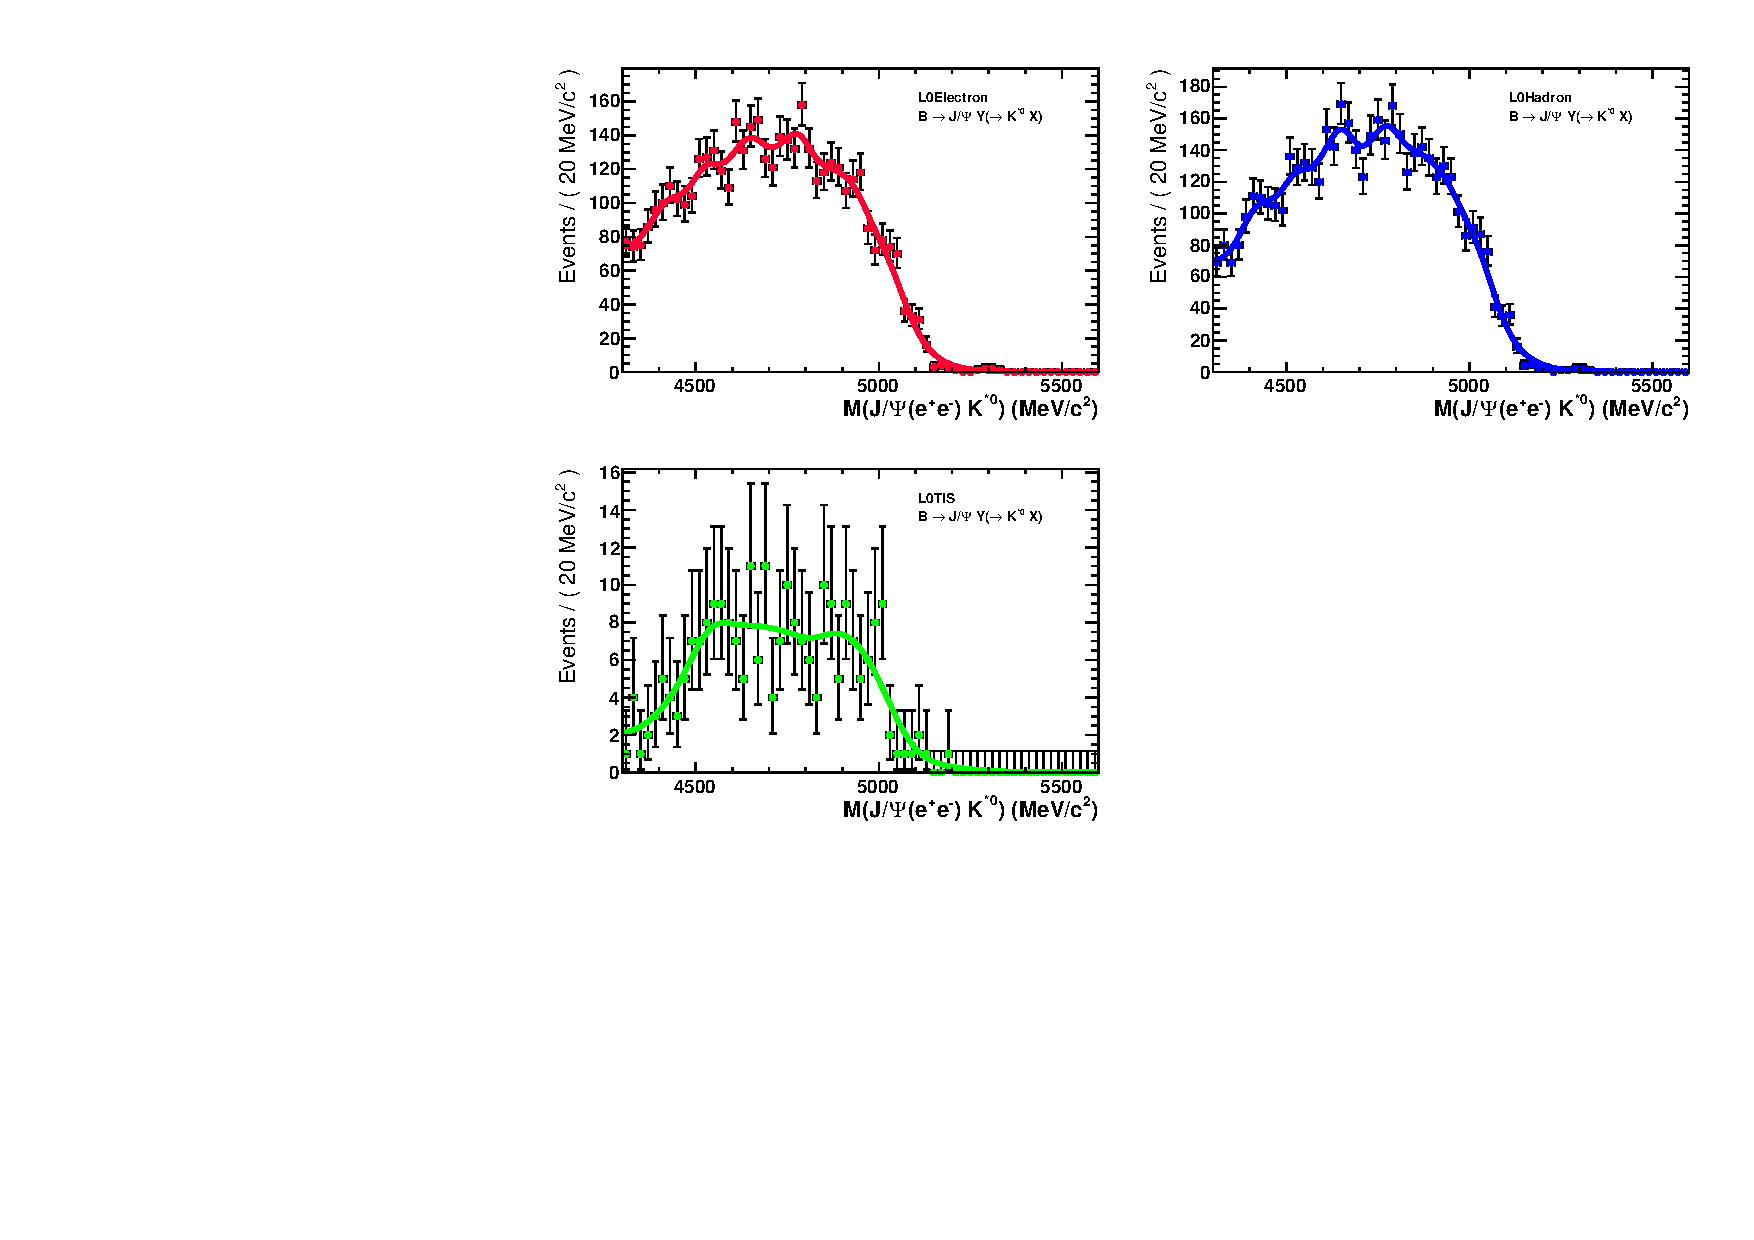
\includegraphics[width = \textwidth]{PartHad.pdf}
\end{center}
\vspace*{-0.8cm}
\caption{\textit{Shapes of the partially reconstructed background from decays of the form $\B \rightarrow \epem Y(\rightarrow \Kstarz X)$ obtained from inclusive Monte Carlo samples for the three trigger categories. The dots represent the data points while the curves are the \PDF described by the \roopdf objects.}}
\label{fig:parthad}
\end{figure}


\begin{figure}[ht]
\vspace*{-0.5cm}
\begin{center}
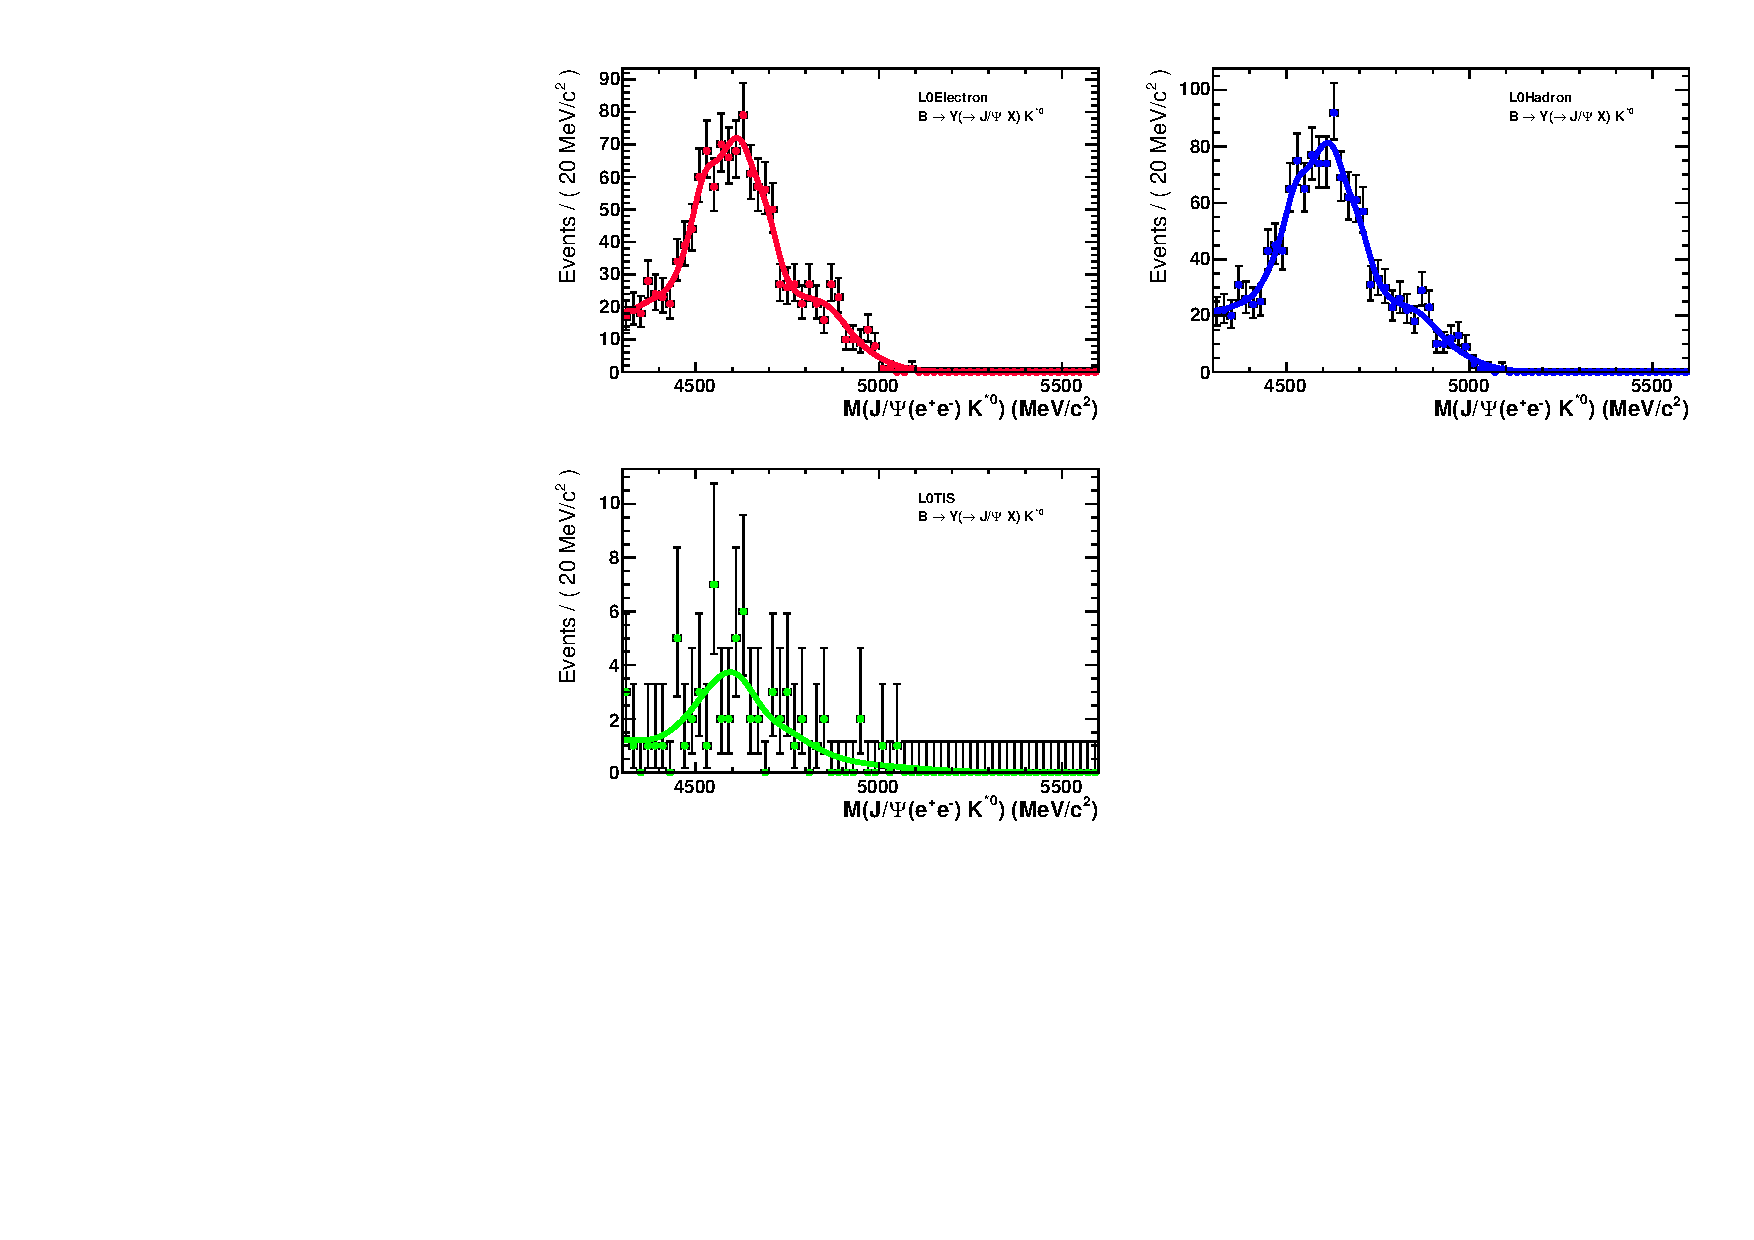
\includegraphics[width = \textwidth]{PartPsi.pdf}
\end{center}
\vspace*{-0.8cm}
\caption{\textit{Shapes of the partially reconstructed background from decays of the form $B \rightarrow (Y \rightarrow \jpsi X) \Kstarz$ obtained from inclusive Monte Carlo samples for the three trigger categories. The dots represent the data points while the curves are the \PDF described by the \roopdf objects.}}
\label{fig:partpsi}
\vspace*{0.5cm}
\end{figure}

\section{Fit strategy and results}
\label{sec:fitstrat}
In this section the fit strategy and means of constraining the parameters of the \PDF for the \BdKstee \lhcb data are presented. To obtain all parameters needed to perform the fit on the \BdKstee \lhcb data information has to be extracted and combined from the \BdKstee Monte Carlo, the \BdToJPsieeKst Monte Carlo and the \BdToJPsieeKst \lhcb data.\\
The \BdToJPsieeKst decay is used in this comparison because it has a much larger yield and the same final state particles. Thus the reconstruction follows using the same detector components and reconstruction algorithms which results in the same effects on the reconstructed \Bd mass shape. Furthermore the same selection as for the \BdKstee can be applied to the \BdToJPsieeKst with exception of the cut on the invariant mass of the electron-positron pair. However, the kinematics are not exactly the same for both decays and therefore it is not possible to rely on information from the \BdToJPsieeKst data only. \\
While the shape of the \BdKstee signal \PDF depends on the kinematics of the decay, the effects from detector resolution and calibration predominately depend on the final state particles. Therefore the \BdKstee Monte Carlo is used to extract information about the shape of the signal, that is the parameters of the double CB distribution while the comparison between the signal \PDF from the \BdToJPsieeKst Monte Carlo with the \BdToJPsieeKst data gives the difference in resolution (effect on the width of the signal \PDF) between Monte Carlo and detector and also the difference in calibration (effect on the mean of the double CB distribution). \\
Additionally to the information about the signal \PDF, the portion of partially reconstructed background events with respect to signal events is extracted from the \BdToJPsieeKst data. This approach relies on the assumption that the amount of $\B \rightarrow \jpsi Y(\rightarrow \Kstarz X)$ events with respect to \BdToJPsieeKst events is the same as the amount of $\B \rightarrow \epem Y(\rightarrow \Kstarz X)$ with respect to \BdKstee events. This assumption can be made because partially reconstructed background concerns only the $Y(\rightarrow \Kstarz X)$ part of the decay. Therefore it is independent of the difference between \BdKstee and \BdToJPsieeKst which is the (\epem) and \jpsi part.\\
This strategy is not applicable to the combinatorial background since the number of combinatorial background events as well as the slope of the exponential describing its \PDF depend on the kinematics of the particles in the decay. This results from the almost random matching of traces in the detector. For example, in order to seemingly form a \jpsi or the \epem pair the combinatorial background electrons have to be selected from different parts of their momentum spectrum. Since this momentum spectrum is not flat and differs from the momentum spectrum of the signal electrons, the number of combinatorial background as well as the slope of the exponential depend on the requirements namely the electron-positron invariant mass.\\
All fits are performed with an extended unbinned maximum likelihood fit.\\

\subsection{The fit to the \BdToJPsieeKst Monte Carlo}
First a double CB distribution like in Equation \ref{eq:dcb} is fitted to the \BdToJPsieeKst Monte Carlo. All fitted parameters are extracted and stored. Figure \ref{fig:jpsimc} shows the \BdToJPsieeKst Monte Carlo and the fitted distribution for the three independent trigger categories.
\begin{figure}[ht]
\vspace*{-0.5cm}
\begin{center}
\subfigure{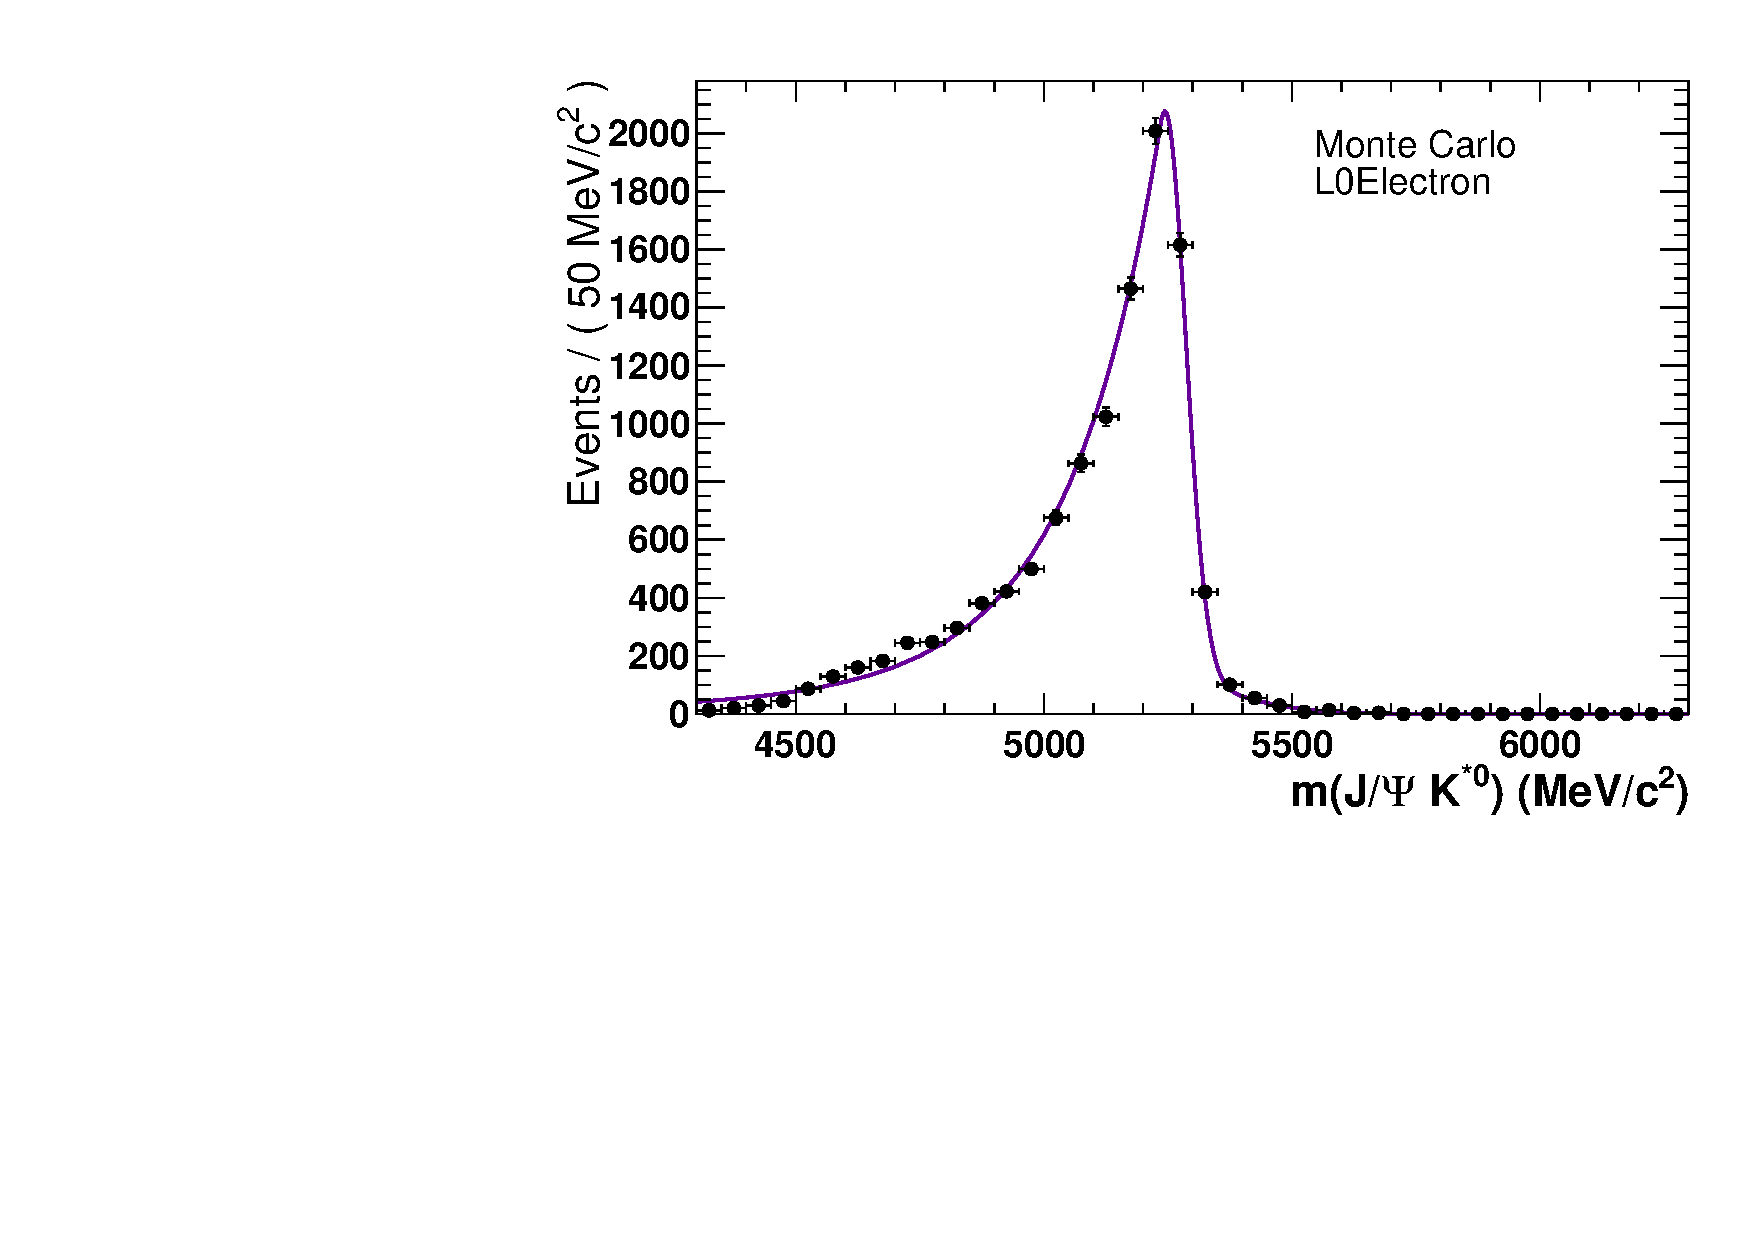
\includegraphics[width = 0.45\textwidth]{MC_L0Ele_JpsiKstar.pdf}}
\subfigure{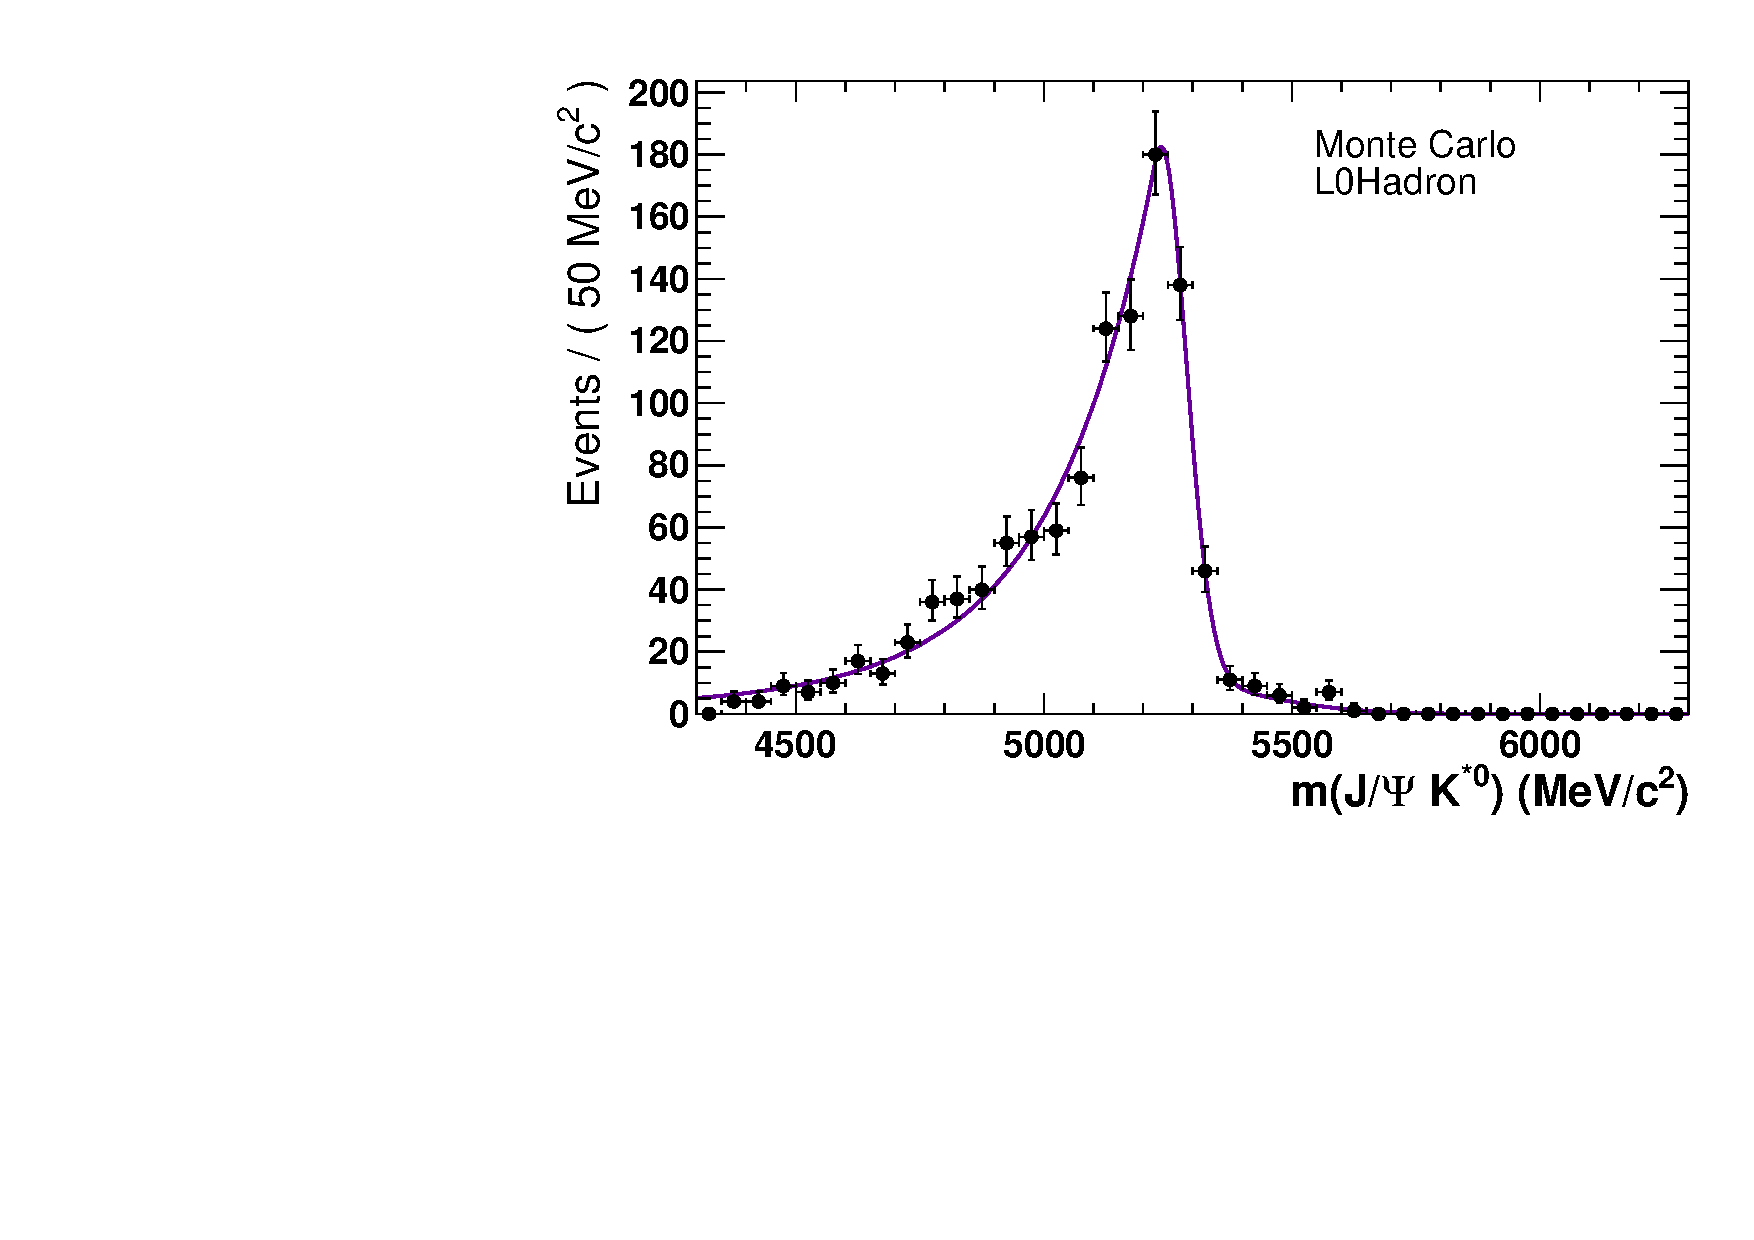
\includegraphics[width = 0.45\textwidth]{MC_L0Had_JpsiKstar.pdf}}\\
\vspace*{-0.5cm}
\subfigure{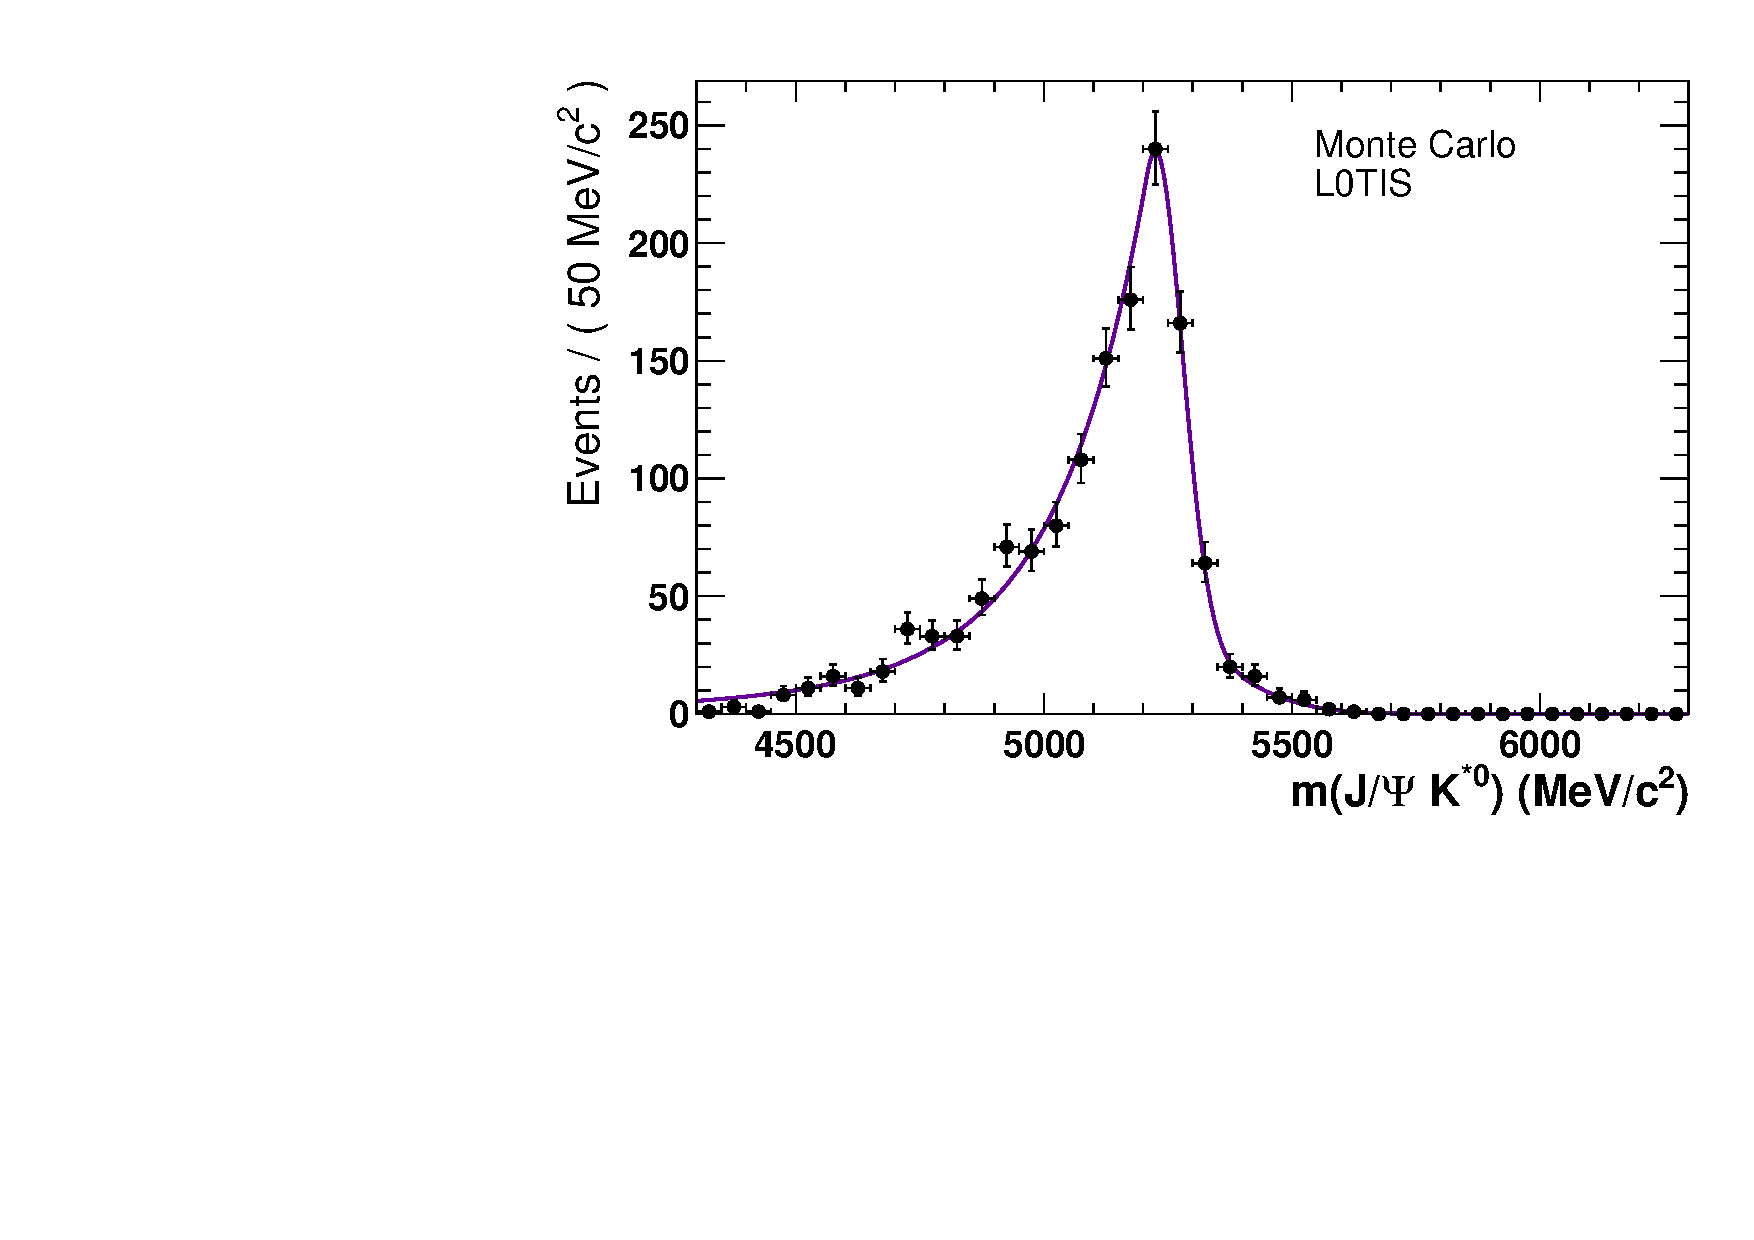
\includegraphics[width = 0.45\textwidth]{MC_L0TIS_JpsiKstar.pdf}}
\end{center}
\vspace*{-1.cm}
\caption{\textit{\BdToJPsieeKst Monte Carlo after the entire selection procedure. The violet curve is the fitted double Crystal-Ball distribution.}}
\label{fig:jpsimc}
\end{figure}

\subsection{Fit to the \BdToJPsieeKst \lhcb data}
A fit to the \BdToJPsieeKst \lhcb data is performed using the \PDF for the signal and the three different background components. In this fit the signal \PDF is constrained by:
\begin{itemize}
\item The parameter $\alpha$ between the two CB distribution is taken from the fit to the \BdToJPsieeKst Monte Carlo.
\item The parameter $n$ is taken from the fit to the \BdToJPsieeKst Monte Carlo.
\item The fraction $f$ is taken from the fit to the \BdToJPsieeKst Monte Carlo.
\item The widths $\sigma_1$ and $\sigma_2$ are taken from the fit to the \BdToJPsieeKst Monte Carlo but are allowed to scale by the same factor $s_{\sigma}$ to account for differences in resolution between the Monte Carlo and \lhcb data (for example due to imperfect detector alignment and/or effects from detector ageing that are not modelled in the Monte Carlo).
\end{itemize}
The mean of the double CB distribution is free.\\
While the slope of the combinatorial background \PDF is free to be fitted as well as the number of combinatorial background events, the number of partially reconstructed background events are fitted with respect to the number of \\ \BdToJPsieeKst signal events for the two types of partially reconstructed background respectively. I.e. the numbers of partially reconstructed background are \\
$N^{part. bkg \Kstarz}_{\jpsi \Kstarz} = r^{part. bkg \Kstarz}_{\jpsi \Kstarz} \cdot N^{sig}_{\jpsi \Kstarz}$ and $N^{part. bkg \jpsi}_{\jpsi \Kstarz} = r^{part. bkg \jpsi}_{\jpsi \Kstarz} \cdot N^{sig}_{\jpsi \Kstarz}$ and the ratios $r^{part. bkg \Kstarz}_{\jpsi \Kstarz}$ and $r^{part. bkg \jpsi}_{\jpsi \Kstarz} $ are fitted.\\

\subsubsection{Contribution from the $\Bs \rightarrow \jpsi (\epem)  \Kstarz$ decay}
The  $\Bs \rightarrow \jpsi (\epem)  \Kstarz$ decay can also occur but at a strongly reduced rate due to the CKM elements involved and due to the smaller production rate of \Bs meson compared to \Bd mesons.\\
All parameters of the double CB distribution for the $\Bs \rightarrow \jpsi (\epem)  \Kstarz$ are taken to be the same as for the \BdToJPsieeKst except for the mean and the number of $\Bs \rightarrow \jpsi (\epem)  \Kstarz$ events. The mean of the $\Bs \rightarrow \jpsi (\epem)  \Kstarz$ distribution is fixed to the mean of \BdToJPsieeKst shifted by $88 \mevcc$\footnote{$m^{PDG}(\Bs) - m^{PDG}(\Bd) = 88\mevcc$}.\\
The ratio of numbers of $\Bs \rightarrow \jpsi (\epem) \Kstarz$ events with respect to \BdToJPsieeKst events was constrained by a Gaussian with mean
 $\mu^{constr.}_{\Bs} = \frac{N_{\Bs}}{N_{\Bd}} = 8.5 \cdot 10^{-3}$ and width $\sigma^{constr.}_{\Bs} = 1.2 \cdot 10^{-3}$.
These values are taken from the analysis of the\\ $\Bs \rightarrow \jpsi (\epem) \Kstarz$ \cite{BsJpsi} where the ratio of events from $\Bs \rightarrow \jpsi (\epem) \Kstarz$ to \BdToJPsieeKst was studied.\\
Figures \ref{fig:jpsidata} shows the \BdToJPsieeKst \lhcb data with the different components of the \PDF.

\begin{figure}[!h]
\vspace*{-0.5cm}
\begin{center}
\subfigure{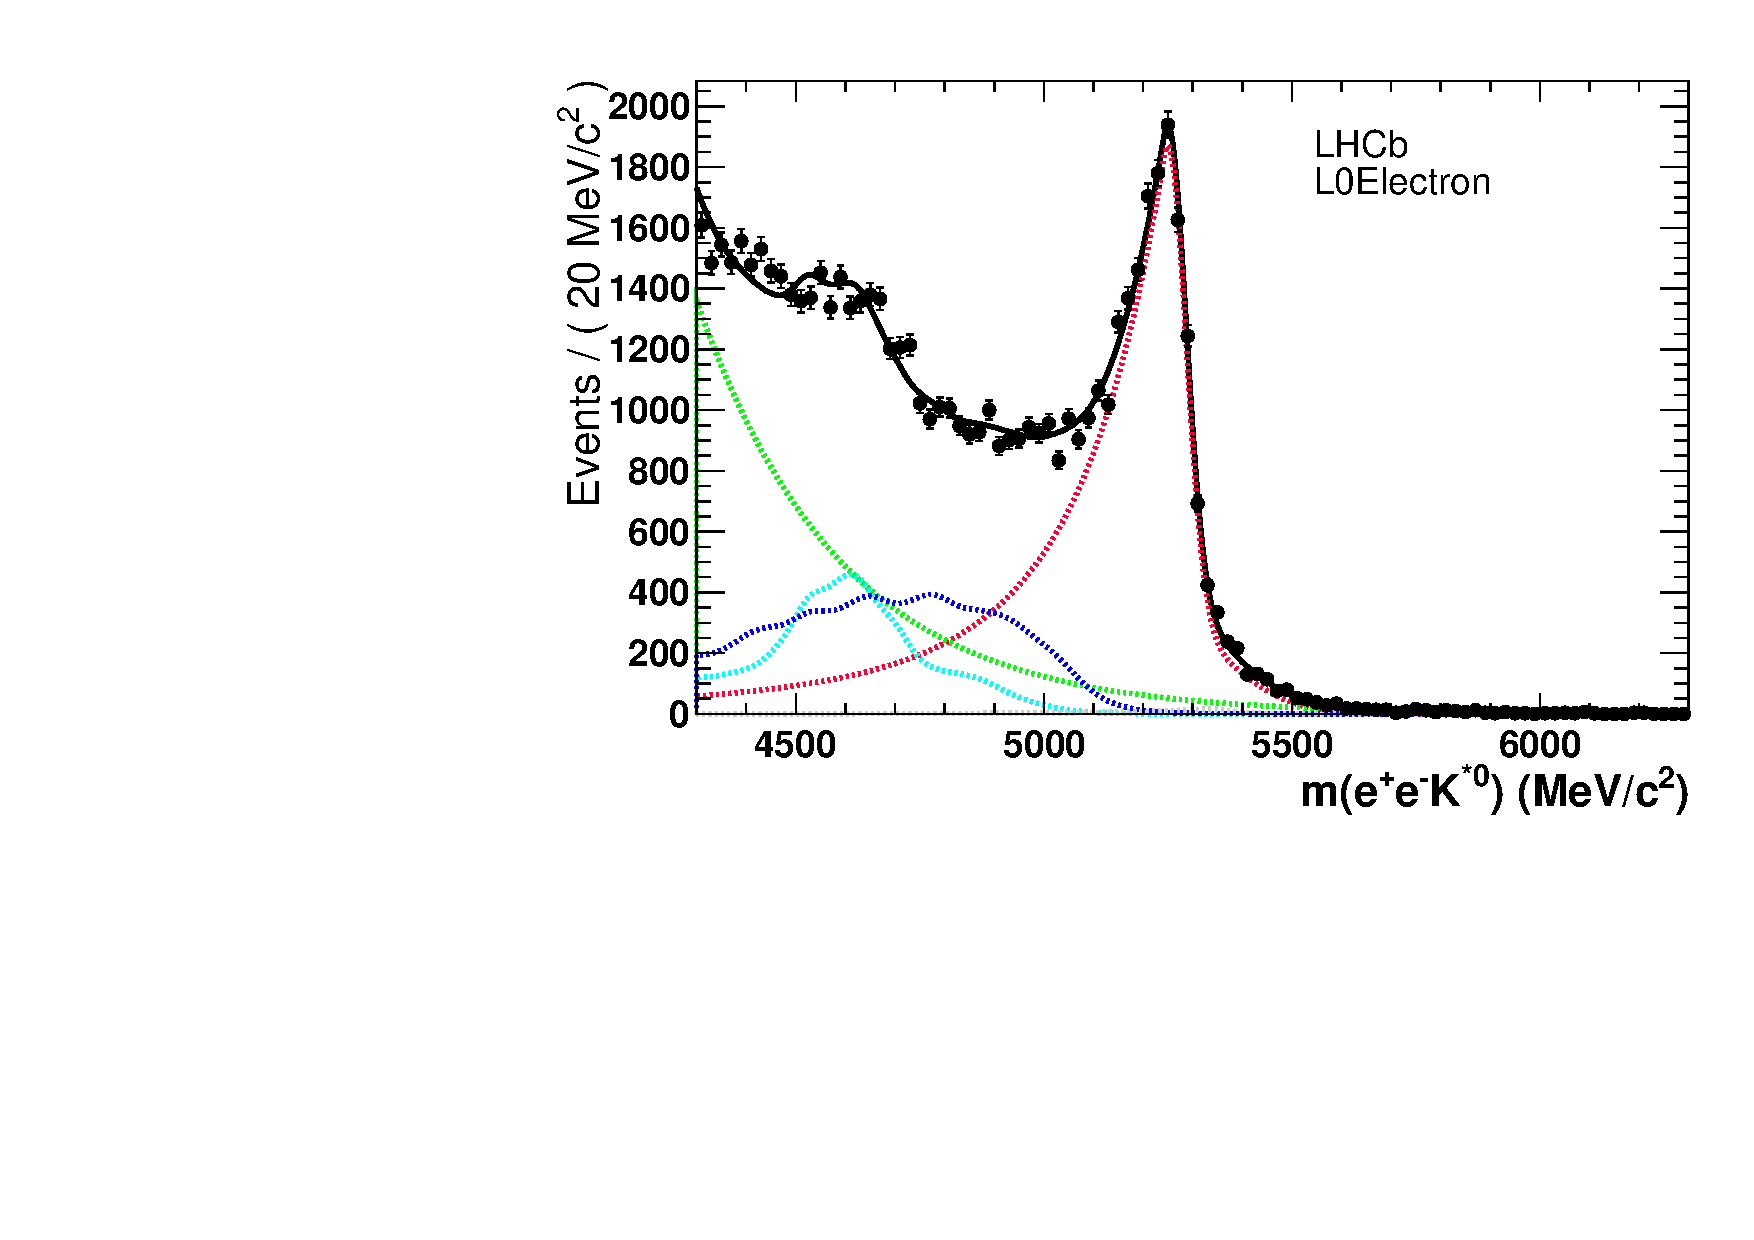
\includegraphics[width = 0.49\textwidth]{Data_L0Ele_JpsiKstar.pdf}}
\subfigure{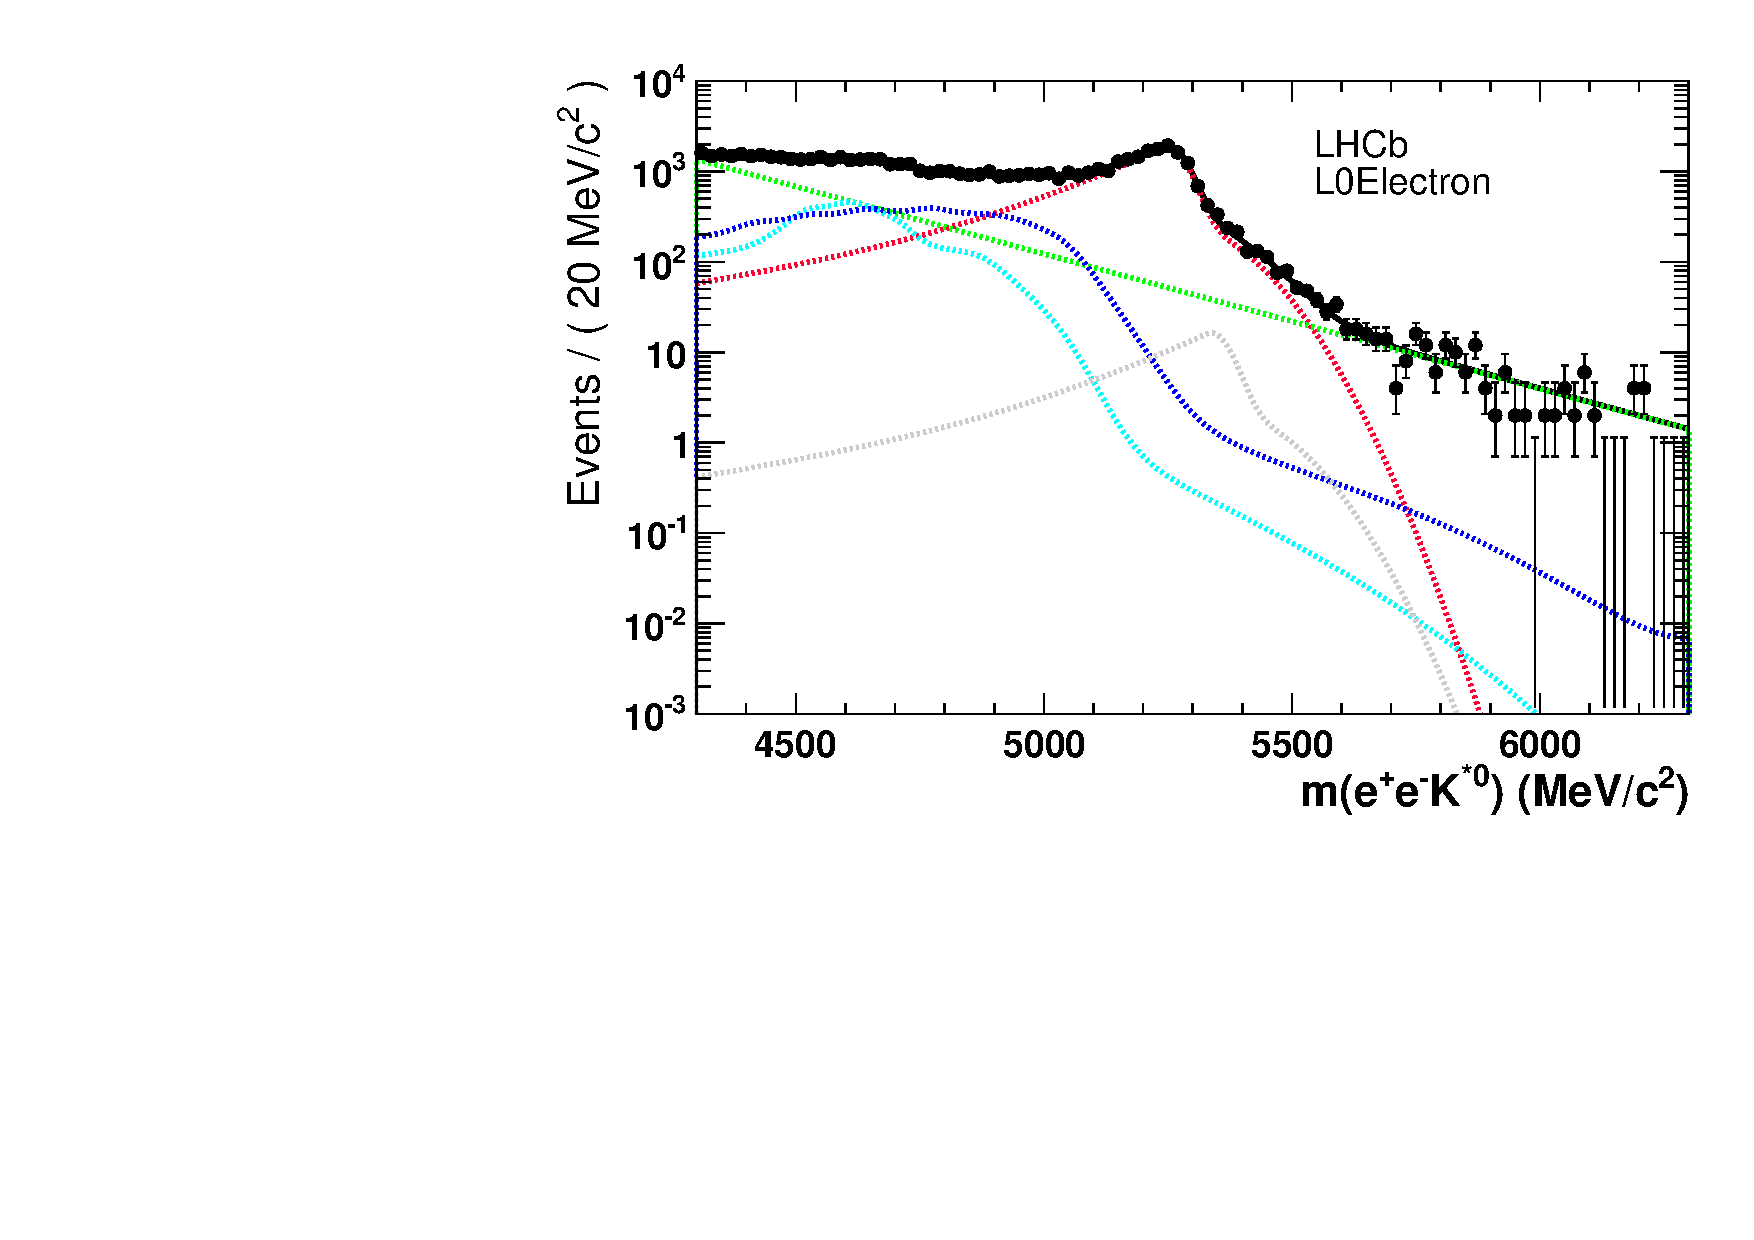
\includegraphics[width = 0.49\textwidth]{LogData_L0Ele_JpsiKstar.pdf}}\\
%\vspace*{-0.5cm}
\subfigure{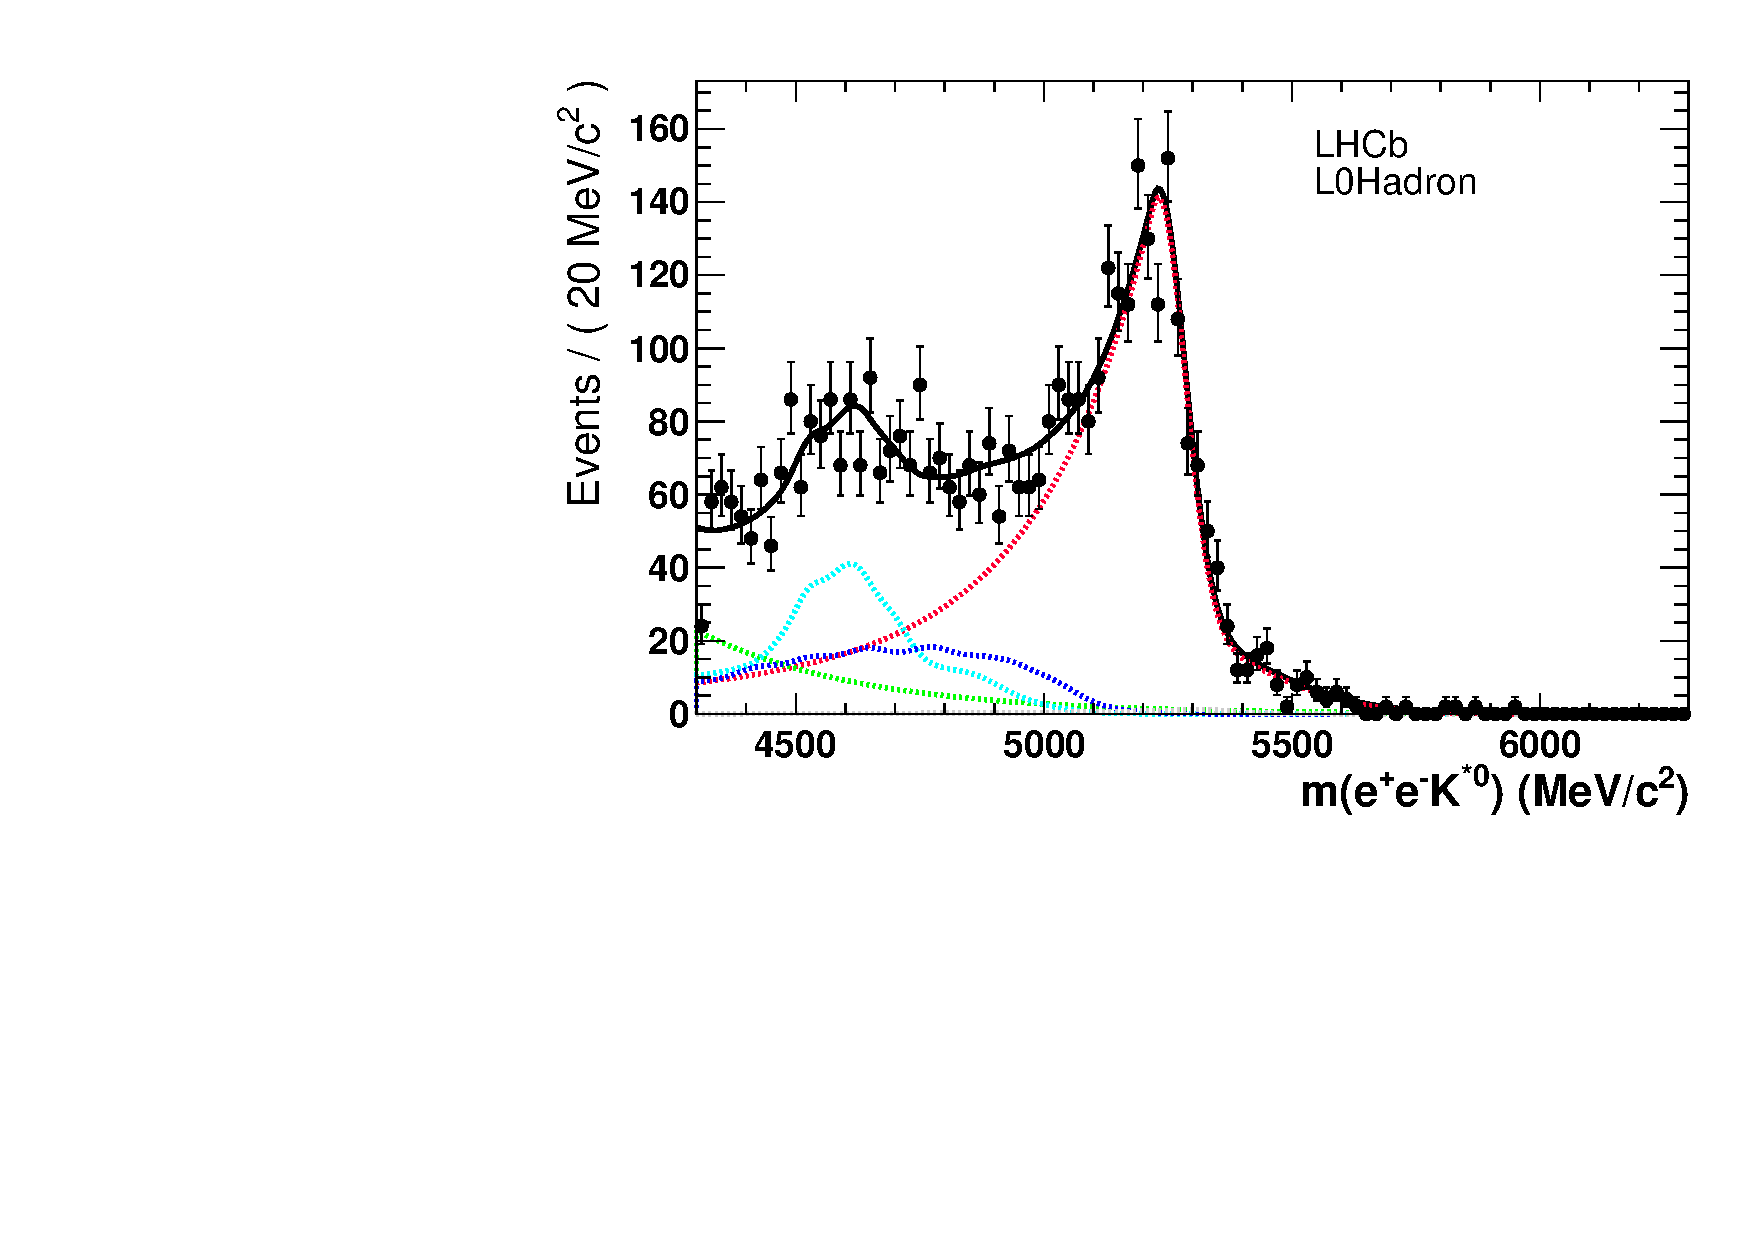
\includegraphics[width = 0.49\textwidth]{Data_L0Had_JpsiKstar.pdf}}
\subfigure{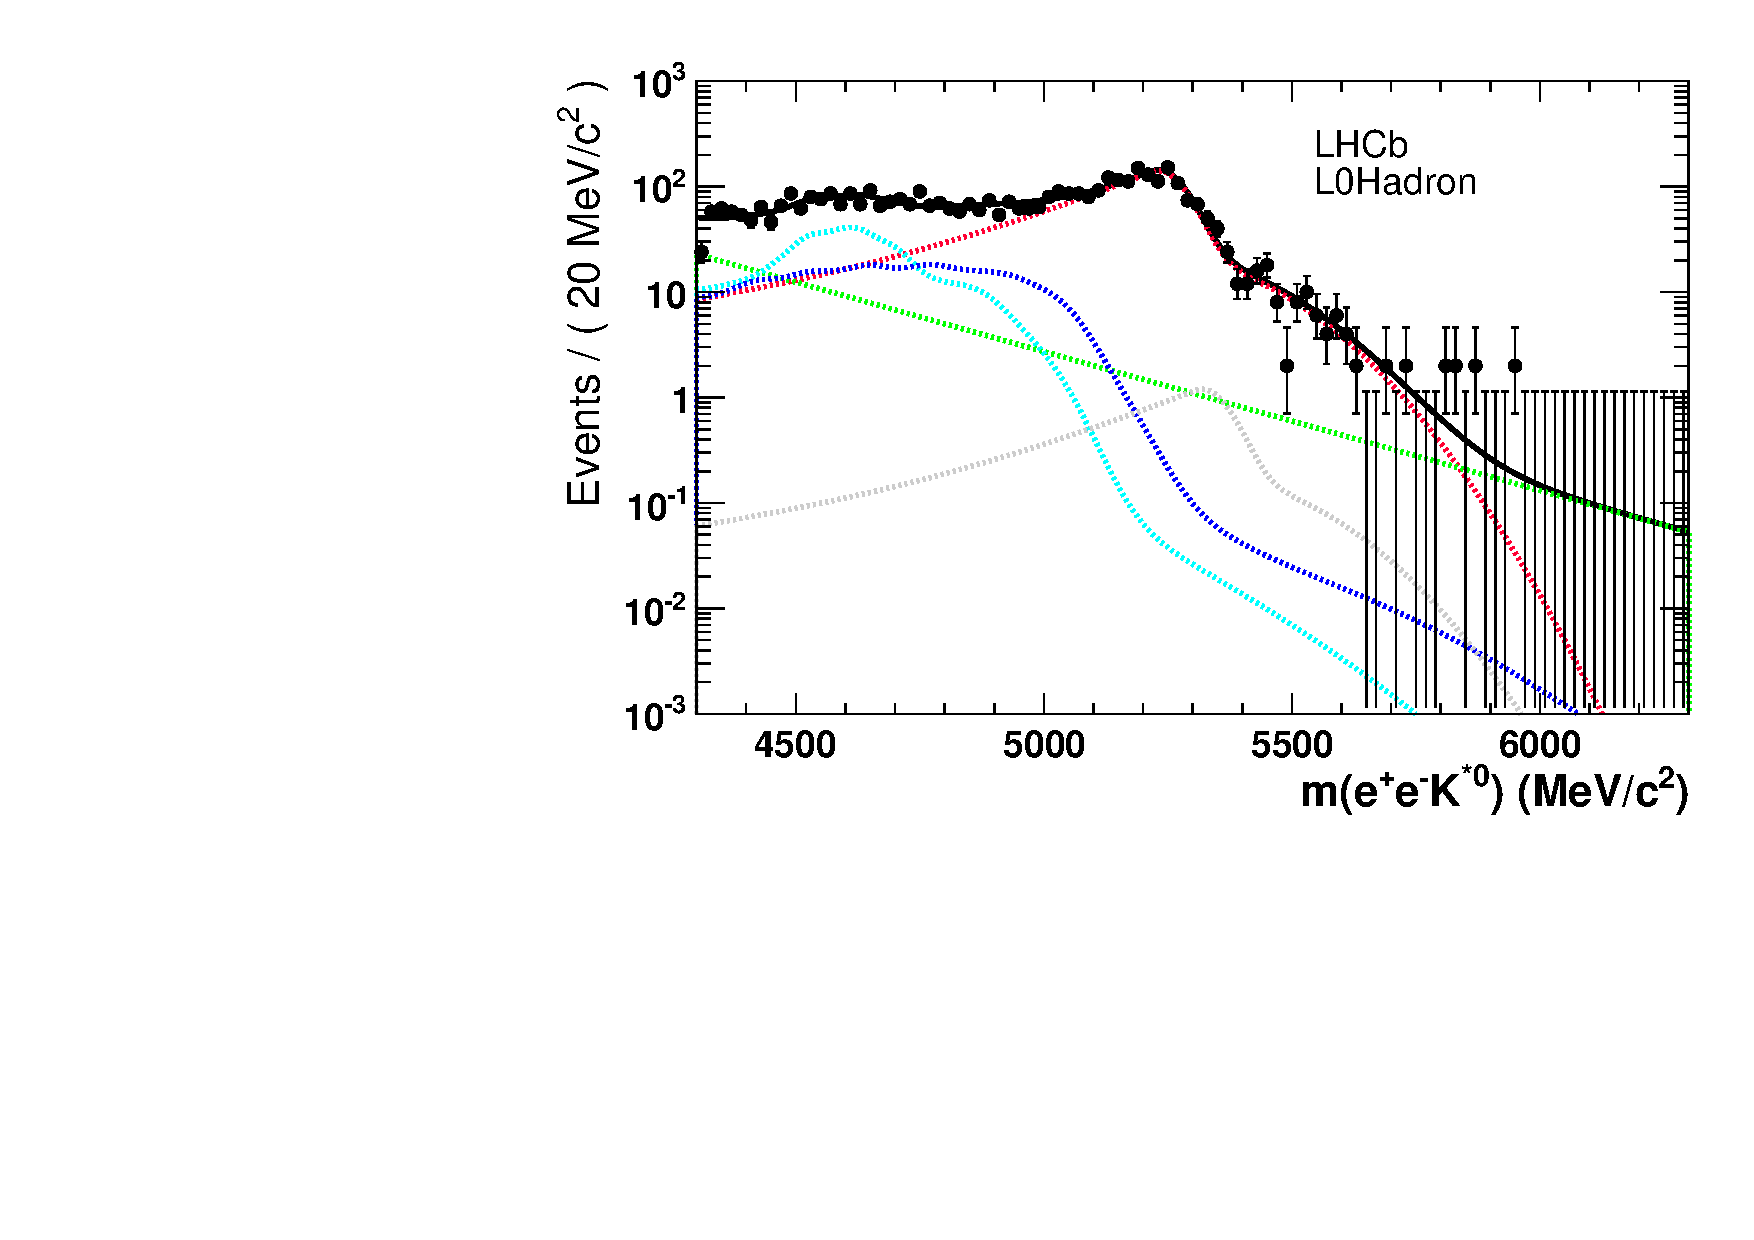
\includegraphics[width = 0.49\textwidth]{LogData_L0Had_JpsiKstar.pdf}}\\
%\vspace*{-0.5cm}
\subfigure{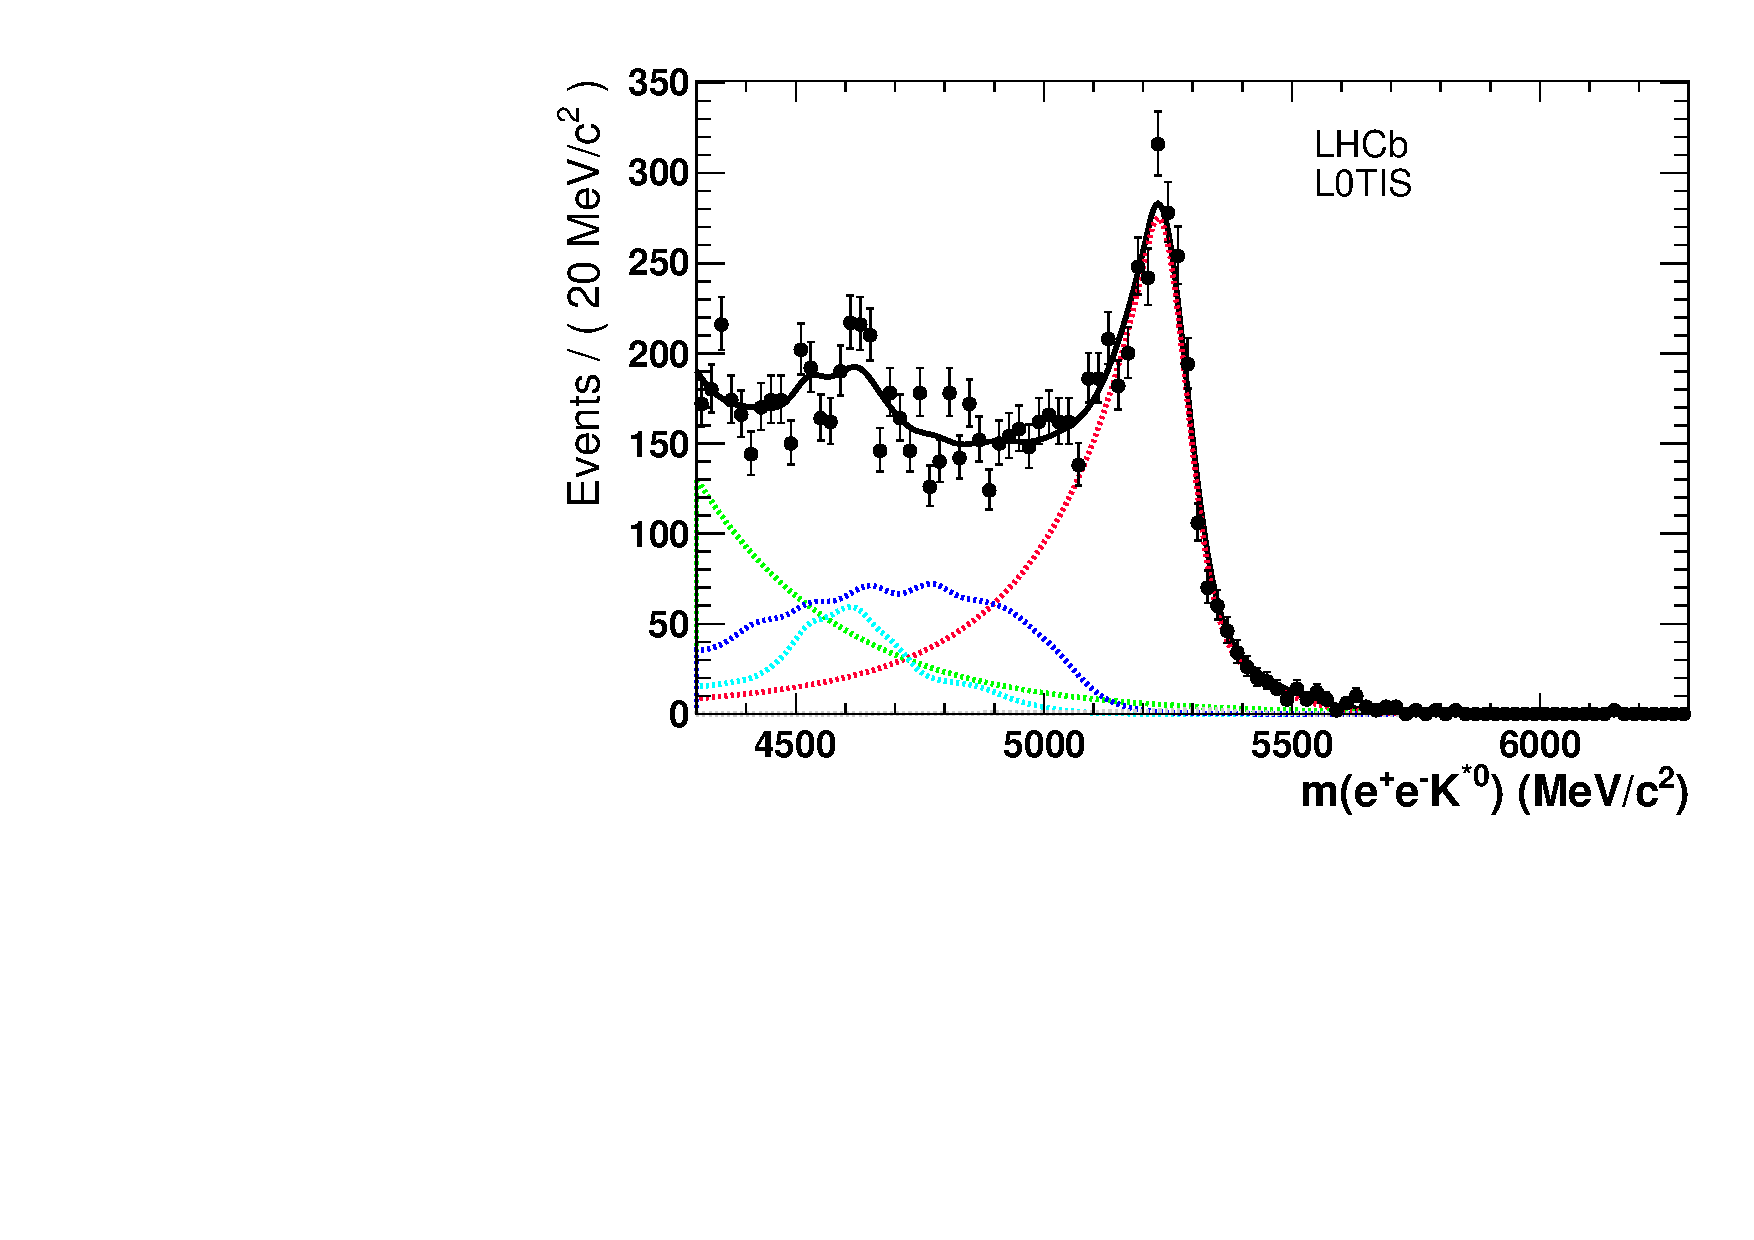
\includegraphics[width = 0.49\textwidth]{Data_L0TIS_JpsiKstar.pdf}}
\subfigure{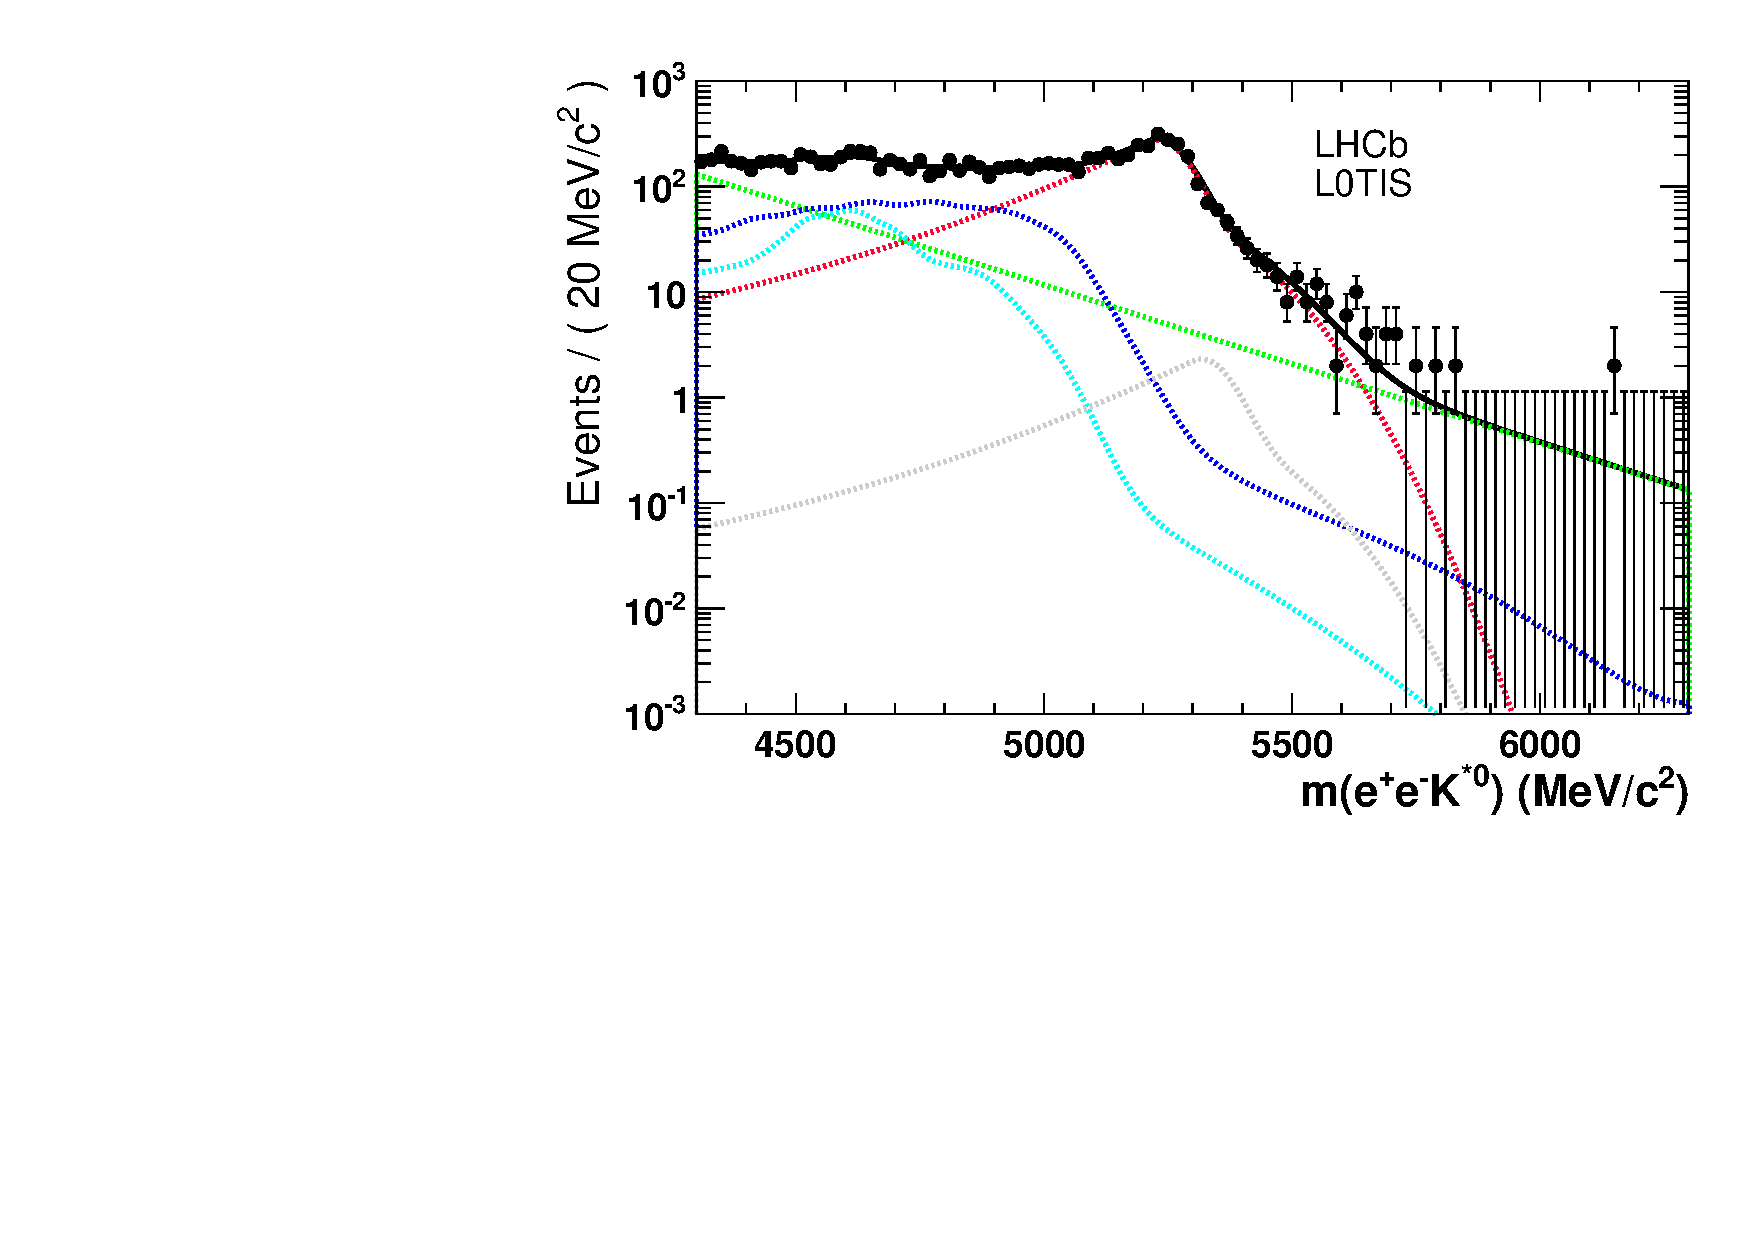
\includegraphics[width = 0.49\textwidth]{LogData_L0TIS_JpsiKstar.pdf}}
\end{center}
%\vspace*{-1cm}
\caption{\textit{\BdToJPsieeKst \lhcb data sample after the entire selection procedure with linear axis on the left and logarithmic axis representation on the right for each trigger category. \textbf{Solid black curve}: the final \PDF , \textbf{dashed pink curve}: the signal \PDF, \textbf{dashed green curve}: the \PDF of the combinatorial background, \textbf{dashed dark blue curve}: the \PDF of the partially reconstructed background of the form $\B \rightarrow \epem Y(\rightarrow \Kstarz X)$, \textbf{dashed clear blue curve}: the \PDF of the partially reconstructed background of the form $B \rightarrow (Y \rightarrow \jpsi X) \Kstarz$, \textbf{dashed gray curve}: the \PDF for the $\Bs \rightarrow \jpsi (\epem) \Kstarz$.}}
\label{fig:jpsidata}
\vspace*{2cm}
\end{figure}


%\begin{figure}[ht]
%\begin{center}
%\subfigure{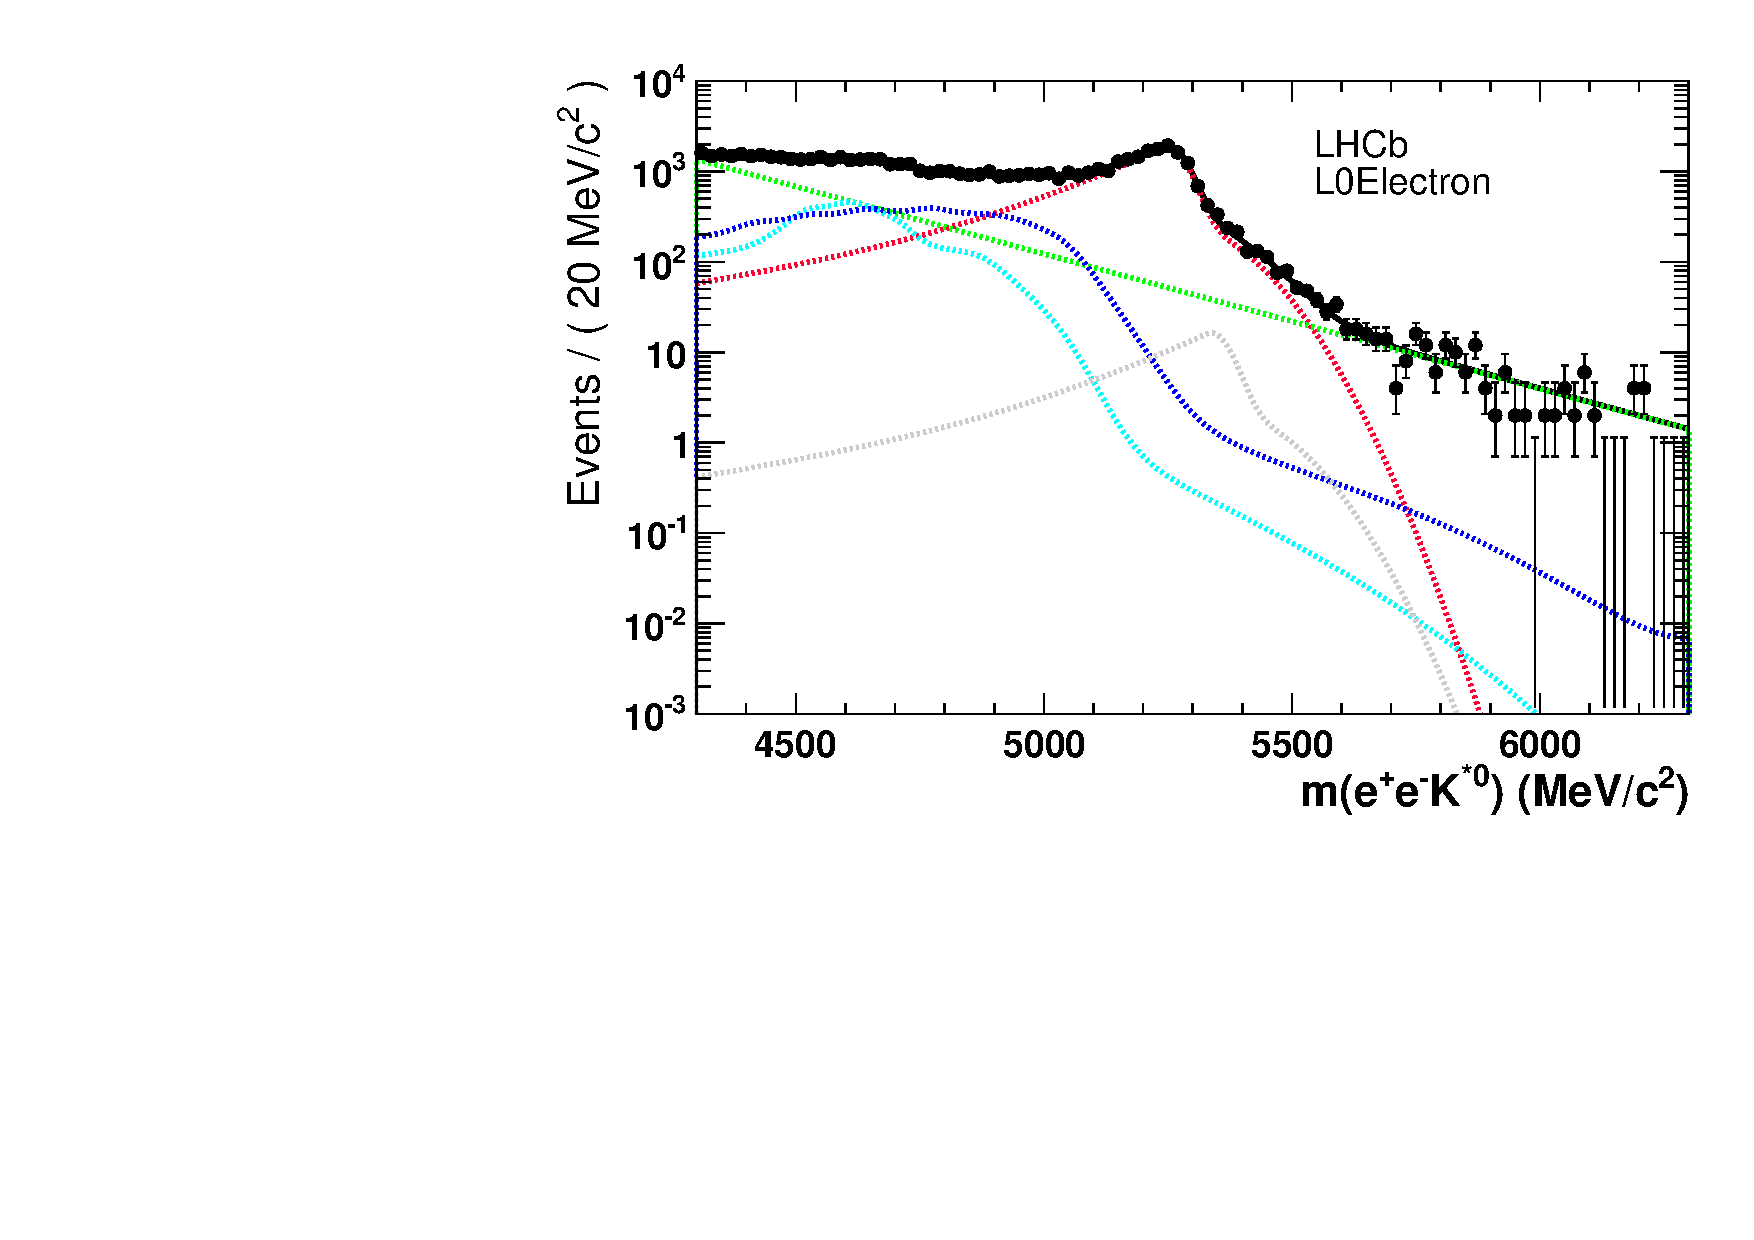
\includegraphics[width = 0.47\textwidth]{LogData_L0Ele_JpsiKstar.pdf}}
%
%\vspace*{-0.5cm}
%
%\end{center}
%\vspace*{-1cm}
%\caption{\textit{\BdToJPsieeKst \lhcb data sample after the entire selection procedure. \textbf{Solid black curve}: the final \PDF , \textbf{dashed pink curve}: the signal \PDF, \textbf{dashed green curve}: the \PDF of the combinatorial background, \textbf{dashed dark blue curve}: the \PDF of the partially reconstructed background of the form $\B \rightarrow \epem Y(\rightarrow \Kstarz X)$, \textbf{dashed clear blue curve}: the \PDF of the partially reconstructed background of the form $B \rightarrow (Y \rightarrow \jpsi X) \Kstarz$, \textbf{dashed gray curve}: the \PDF for the $\Bs \rightarrow \jpsi (\epem) \Kstarz$.}}
%\label{fig:jpsidatalog}
%\end{figure}


\subsection{Fit to the \BdKstee \lhcb data}
In the fit to the \BdKstee \lhcb data only three parameters are left entirely free: the number of signal events $N^{sig}$, the number of combinatorial background events $N^{comb. bkg}$ and the slope $b$ of the exponential function representing the combinatorial background. All other parameters are constrained:
\begin{itemize}
\item Parameters $\boldsymbol{\alpha}$, $\mathbf{n}$, $\mathbf{f}$: parameters of the signal \PDF taken from the double CB distribution fitted to the \BdKstee Monte Carlo.
\item $\mathbf{s_{\boldsymbol{\sigma}}\cdot \boldsymbol{\sigma_1}}$ and $\mathbf{s_{\boldsymbol{\sigma}}\cdot \boldsymbol{\sigma}_2}$: widths of the signal \PDF, $\sigma_1$ and $\sigma_2$ are taken from the double CB distribution fitted to the \BdKstee Monte Carlo, the scale factor $s_{\sigma}$ is taken from the fit to the \BdToJPsieeKst \lhcb data.
\item $\mathbf{\boldsymbol{\mu}^{data}_{\epem \Kstarz}}$: mean of the signal \PDF, is taken to be the mean of the double CB distribution fitted to the \BdToJPsieeKst \lhcb data summed by the difference $\delta_{MC}$ of the mean of the double CB distributions fitted to\\ \BdKstee and \BdToJPsieeKst Monte Carlo \\ $\delta_{MC} = \mu^{MC}_{\epem \Kstarz} - \mu^{MC}_{\jpsi \Kstarz}$.
\item $\mathbf{N^{part. bkg}}$: the number of partially reconstructed background events is indirectly constrained through the Gaussian constraint put on the ratio $r^{part. bkg}\cdot \frac{N^{part. bkg}}{N^{sig}}$. The mean of this Gaussian constraint is taken from the\\ \BdToJPsieeKst \lhcb data fit to be $r^{part. bkg \Kstarz}_{\jpsi \Kstarz}$ and the width is the error on this parameter.\\
\end{itemize}

\subsubsection{Contamination from \BdKstGam events}
In the 2011 analysis the contribution from the \BdKstGam decays had to be taken into account during the fit. However, using the new reconstruction tools presented in Chapter \ref{chapter3} the \BdKstGam contamination is reduced to the level of 1\% and below depending on the trigger category. Therefore contribution from \BdKstGam decays is neglected. The percentage of \BdKstGam events with respect to \BdKstee events was calculated on the Monte Carlo samples and the results are listed in Table \ref{tab:kstgam}.
\renewcommand{\arraystretch}{1.5} 
\begin{table}[ht]
\begin{center}
\begin{tabular}{l |c}
trigger category & \BdKstGam pollution \\
\hline \hline
L0Electron & 1.1\% \\
\hline
L0Hadron & 0.8\% \\
\hline
L0TIS & 0.0\% \\
\end{tabular}
\end{center}
\caption{\textit{Percentage of \BdKstGam events with respect to \BdKstee events after the entire selection determined on Monte Carlo samples.}}
\label{tab:kstgam}
\end{table}
\newpage
Figures \ref{fig:eedata} show the \BdKstee \lhcb data with the different components of the \PDF.
\begin{figure}[ht]
\begin{center}
\subfigure{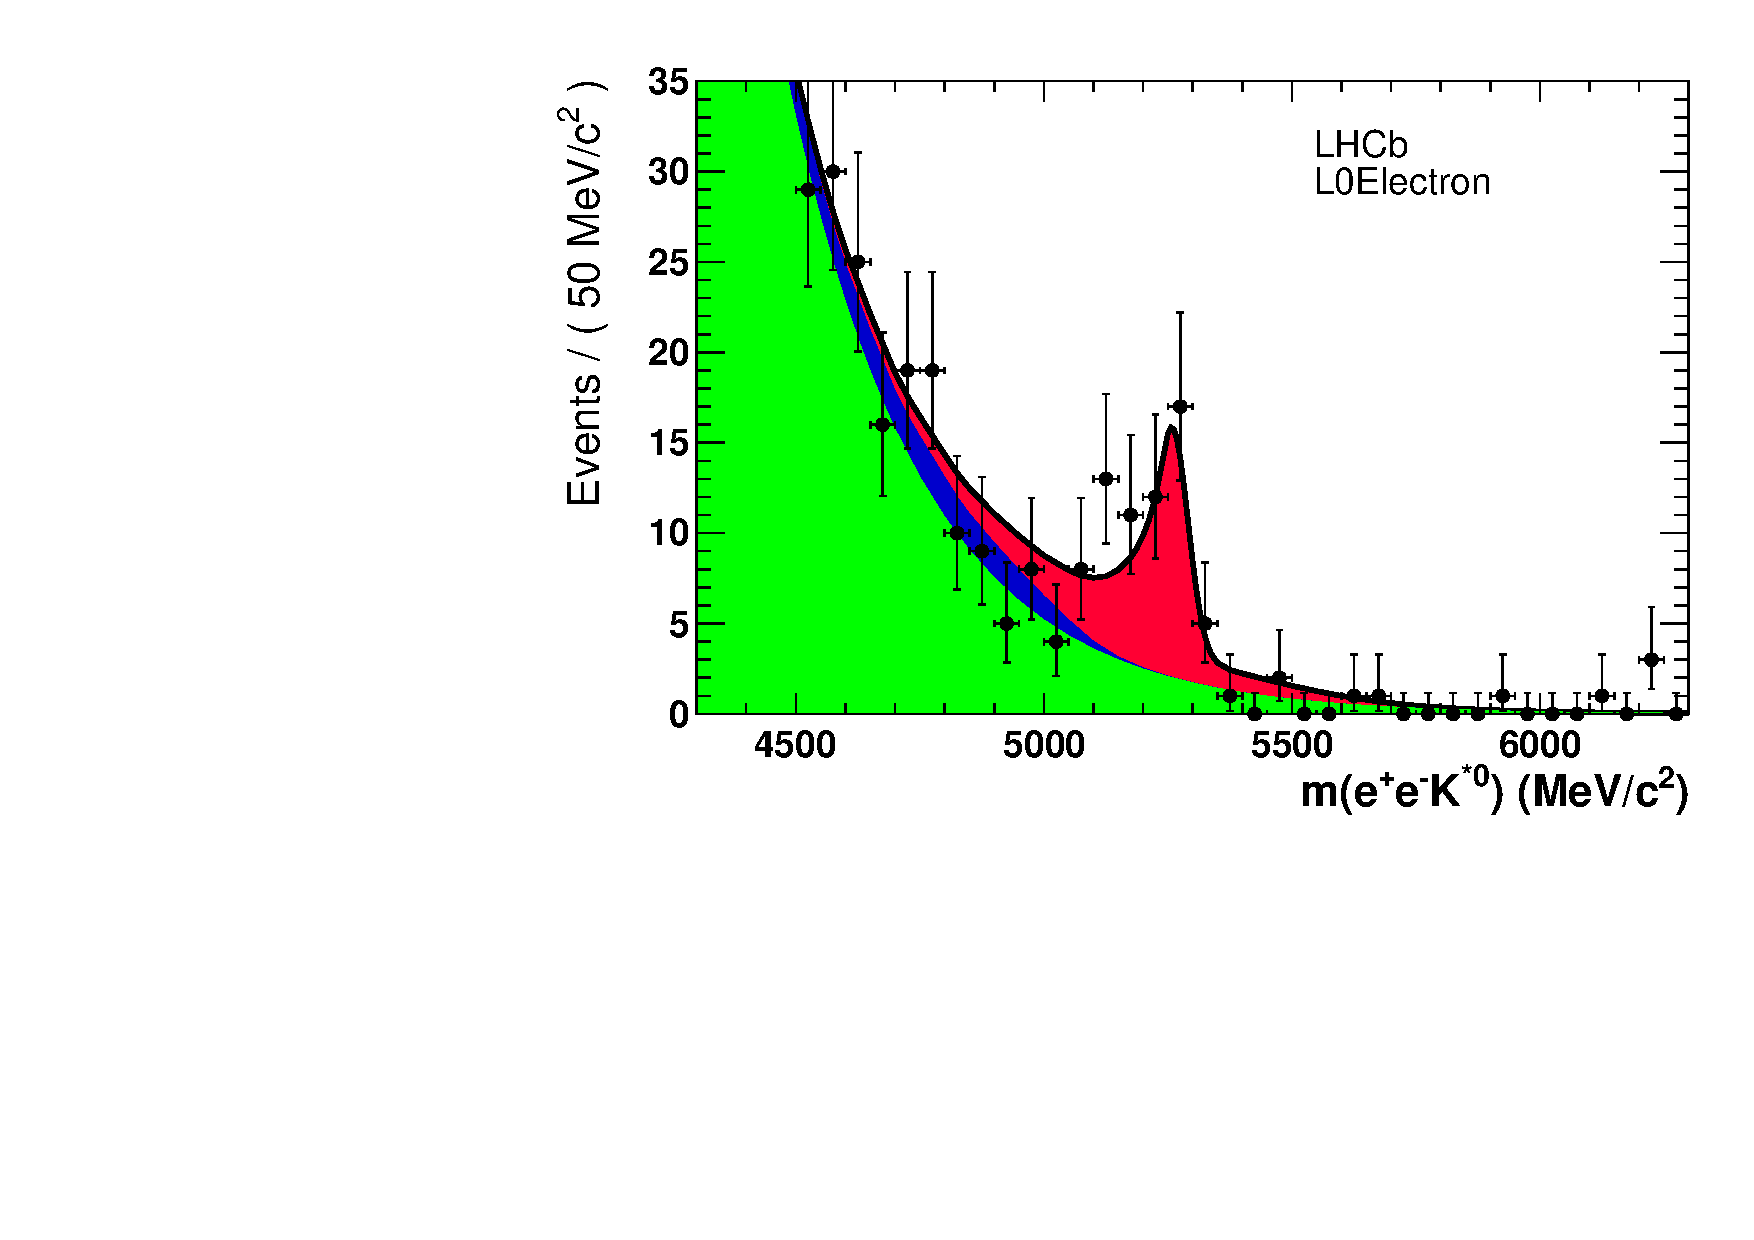
\includegraphics[width = 0.49\textwidth]{40_Data_L0Ele_eeKstar.pdf}}
\subfigure{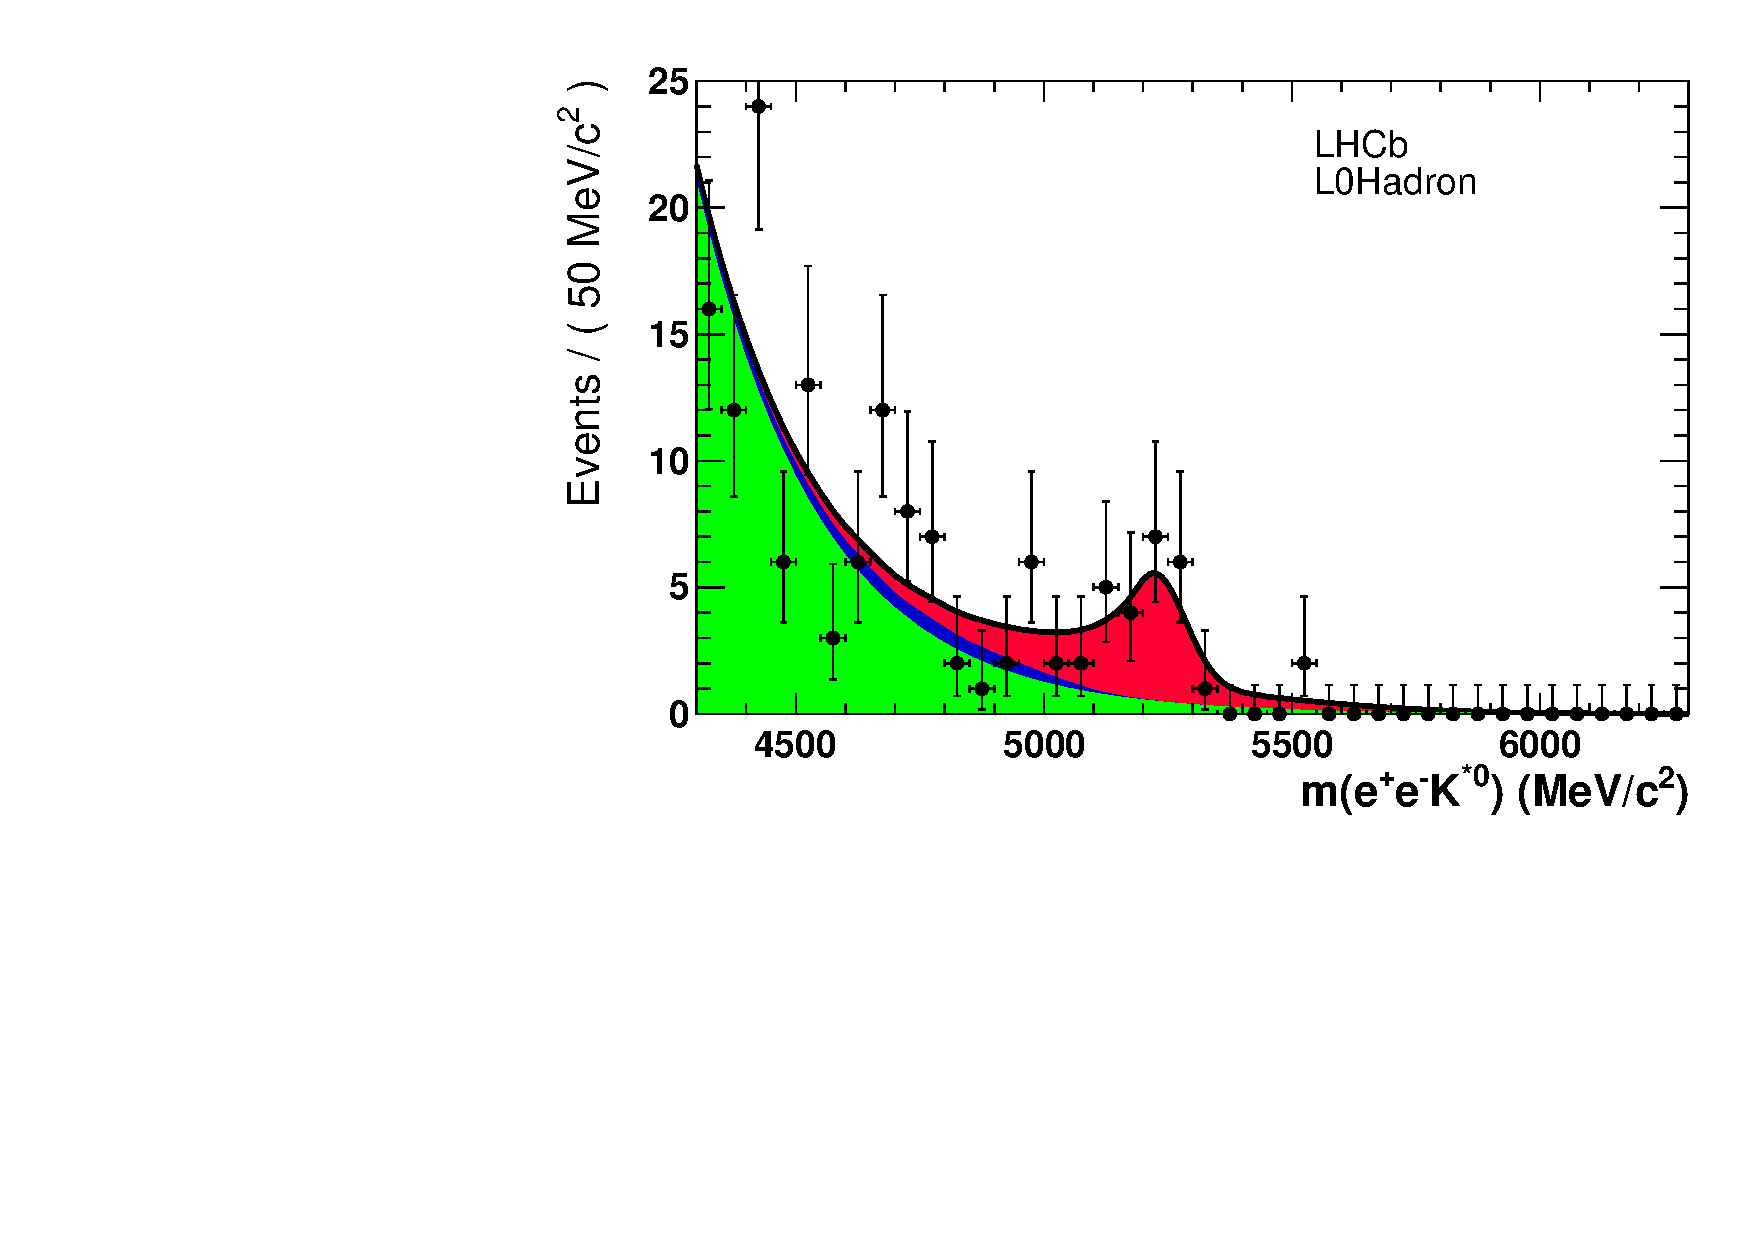
\includegraphics[width = 0.49\textwidth]{40_Data_L0Had_eeKstar.pdf}}\\
\vspace*{-0.5cm}
\subfigure{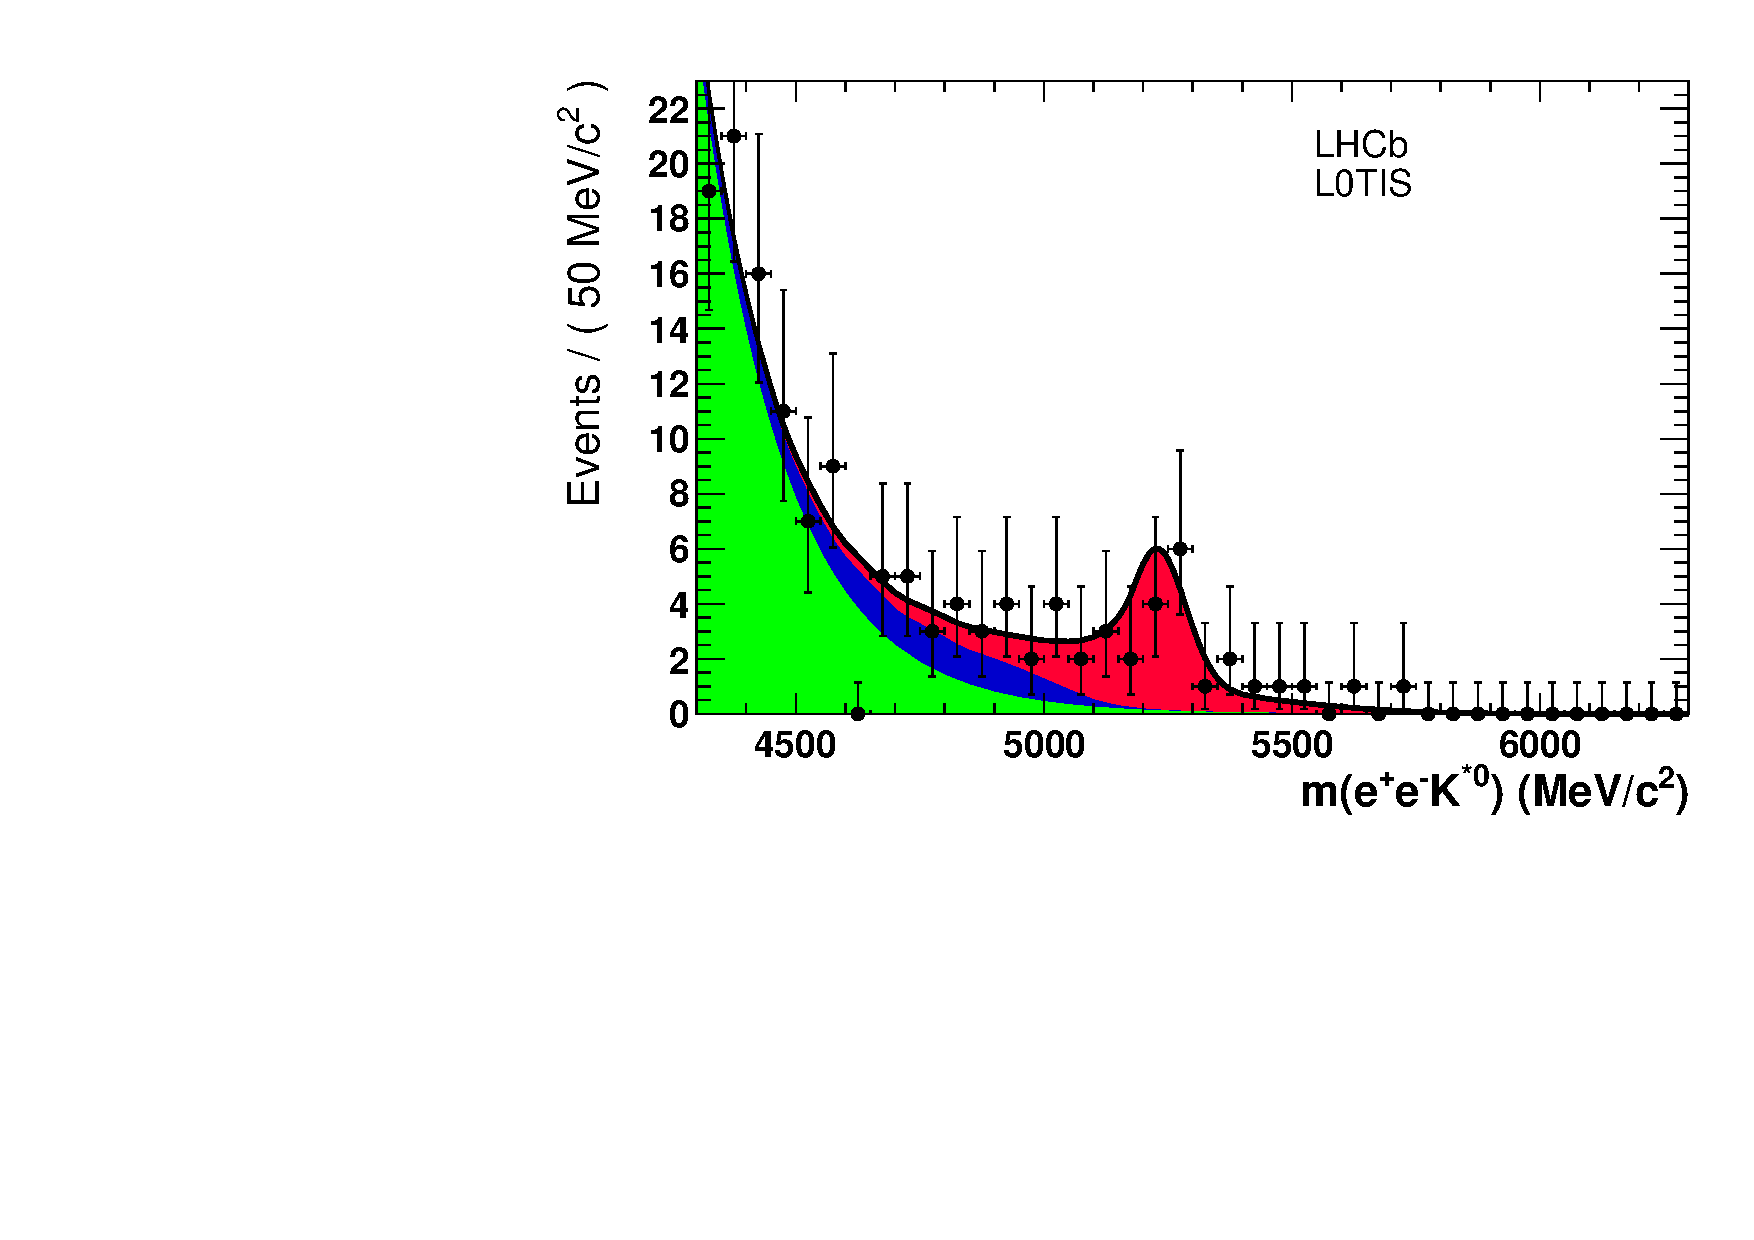
\includegraphics[width = 0.49\textwidth]{40_Data_L0TIS_eeKstar.pdf}}
\end{center}
\vspace*{-0.5cm}
\caption{\textit{\BdKstee \lhcb data after the entire selection procedure. \textbf{Green area}: combinatorial background events, \textbf{blue area}: partially reconstructed background events, \textbf{pink area}: \BdKstee signal events.}}
\label{fig:eedata}
\end{figure}
\\


%\section{Determination of the parameters for the \BdKstee \lhcb data \PDF}
%\label{sec:paramextra}
%In this section it is described how the parameters for the \BdKstee \lhcb data \PDF are extracted from the \BdKstee Monte Carlo, the \BdToJPsieeKst Monte Carlo and the \BdToJPsieeKst \lhcb data.
%
%The signal-function that is fitted to the \BdKstee \lhcb data is:
%\begin{eqnarray}
%\PDF^{sig} \ = & &N^{sig} \left[ \ f\ CB(x;\alpha,n,\mu^{data}_{\jpsi \Kstarz}+ \delta^{MC},s_{\sigma} \cdot \sigma_1) \\
%& +& (1-f)\ CB(x;\alpha,n,\mu^{data}_{\jpsi \Kstarz} + \delta^{MC},s_{\sigma} \cdot \sigma_2) \right]
%\end{eqnarray}
%where all parameters except for the number of signal events $N^{sig}$  are determined in advance:
%\begin{enumerate}
%\item $\boldsymbol{\alpha}$, $\mathbf{n}$, $\mathbf{f}$, $\mathbf{\boldsymbol{\sigma}_1}$ and $\mathbf{\boldsymbol{\sigma}_2}$: parameters of the double CB distribution fitted to the \BdKstee Monte Carlo
%\item $\mathbf{\boldsymbol{\mu}^{data}_{\jpsi \Kstarz}}$: mean of the double CB distribution fitted to the \BdToJPsieeKst \lhcb data
%\item $\mathbf{\boldsymbol{\delta}^{MC}}$: difference between the means of the double CB distributions fitted to the \BdKstee Monte Carlo and the \BdToJPsieeKst Monte Carlo respectively
%\item $\mathbf{s_{\boldsymbol{\sigma}}}$: scale between the widths of the CB distributions fitted to the \BdToJPsieeKst Monte Carlo and \BdToJPsieeKst \lhcb data
%\end{enumerate}
%\\
%The function for the combinatorial background that is fitted to the \BdKstee \lhcb data is:
%\begin{equation}
%\PDF^{comb. bkg} \ = N^{comb. bkg} \cdot e^{bx}
%\end{equation}
%both the number of combinatorial background events $N^{comb. bkg}$ and the slope of the exponential function $b$ are free in the fit.\\
%\\
%The function for the partially reconstructed background of the form $\B \rightarrow \epem Y(\rightarrow \Kstarz X)$ that is fitted to the \BdKstee \lhcb data is:
%\begin{equation}
%\PDF^{comb. bkg} \ = N^{sig}\cdot r^{part. bkg} \cdot \roopdf
%\end{equation}
%where $r^{part. bkg}$ is the ratio of partially reconstructed background events with respect to the number of signal events. This ratio constrained in the fit by the means of a Gaussian constrained. The parameters of this constraining Gaussian are determined from the \BdToJPsieeKst \lhcb data fit and the mean of Gaussian $\mu^{constr.} = \frac{N^{part. bkg}_{\jpsi \Kstarz}}{N^{sig}_{\jpsi \Kstarz}}$ and the width $\sigma^{constr.}$ is the error on the value of $\frac{N^{part. bkg}_{\jpsi \Kstarz}}{N^{sig}_{\jpsi \Kstarz}}$.
%
%
%\section{Fit results}
%\label{sec:fitresults}
%\subsection{\BdToJPsieeKst Monte Carlo}
%Figure \ref{fig:jpsimc} shows the \BdToJPsieeKst Monte Carlo distribution with the double CB distribution fitted to it.
%
%\subsection{\BdKstee Monte Carlo}
%Figure \ref{fig:eemc} shows the \BdKstee Monte Carlo distribution with the double CB distribution fitted to it.
%\begin{figure}[ht]
%\begin{center}
%\subfigure{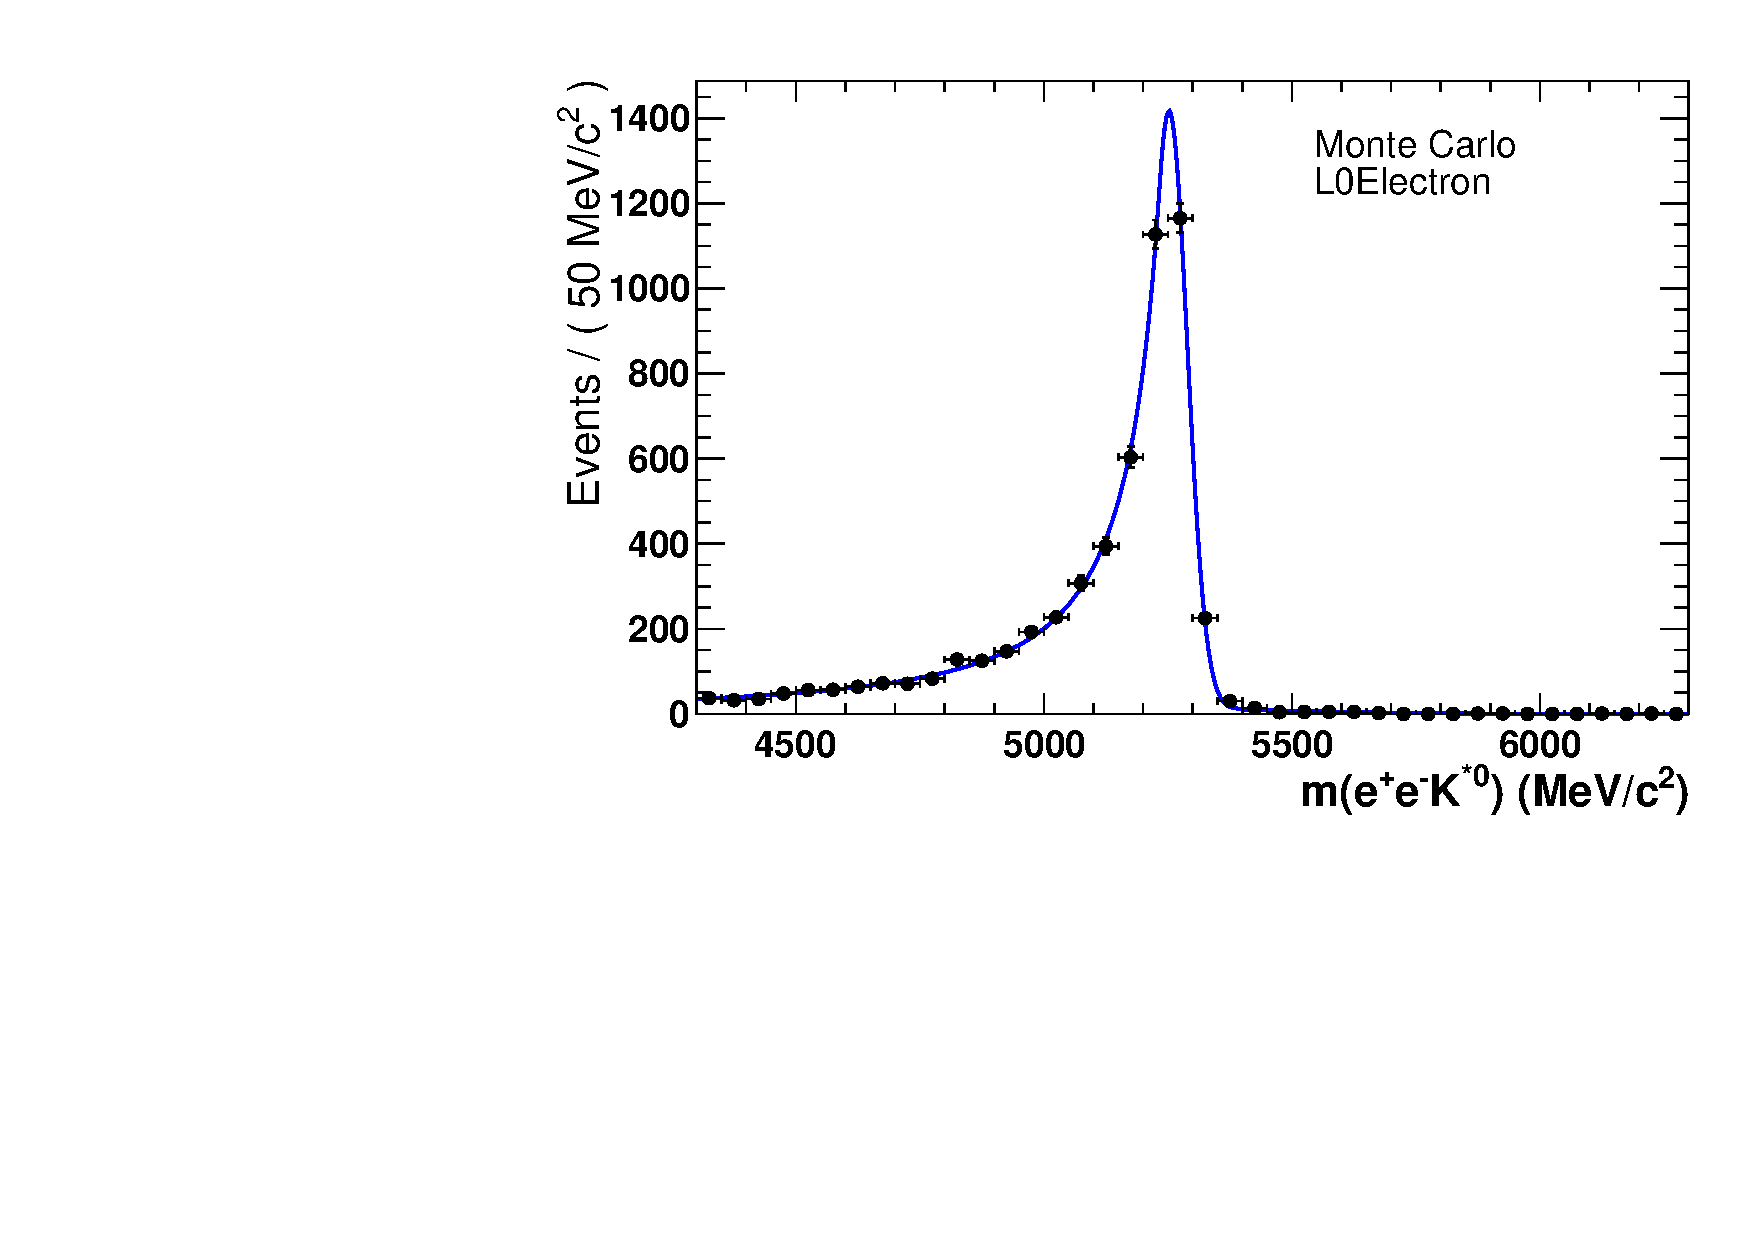
\includegraphics[width = 0.49\textwidth]{MC_L0Ele_eeKstar.pdf}}
%\subfigure{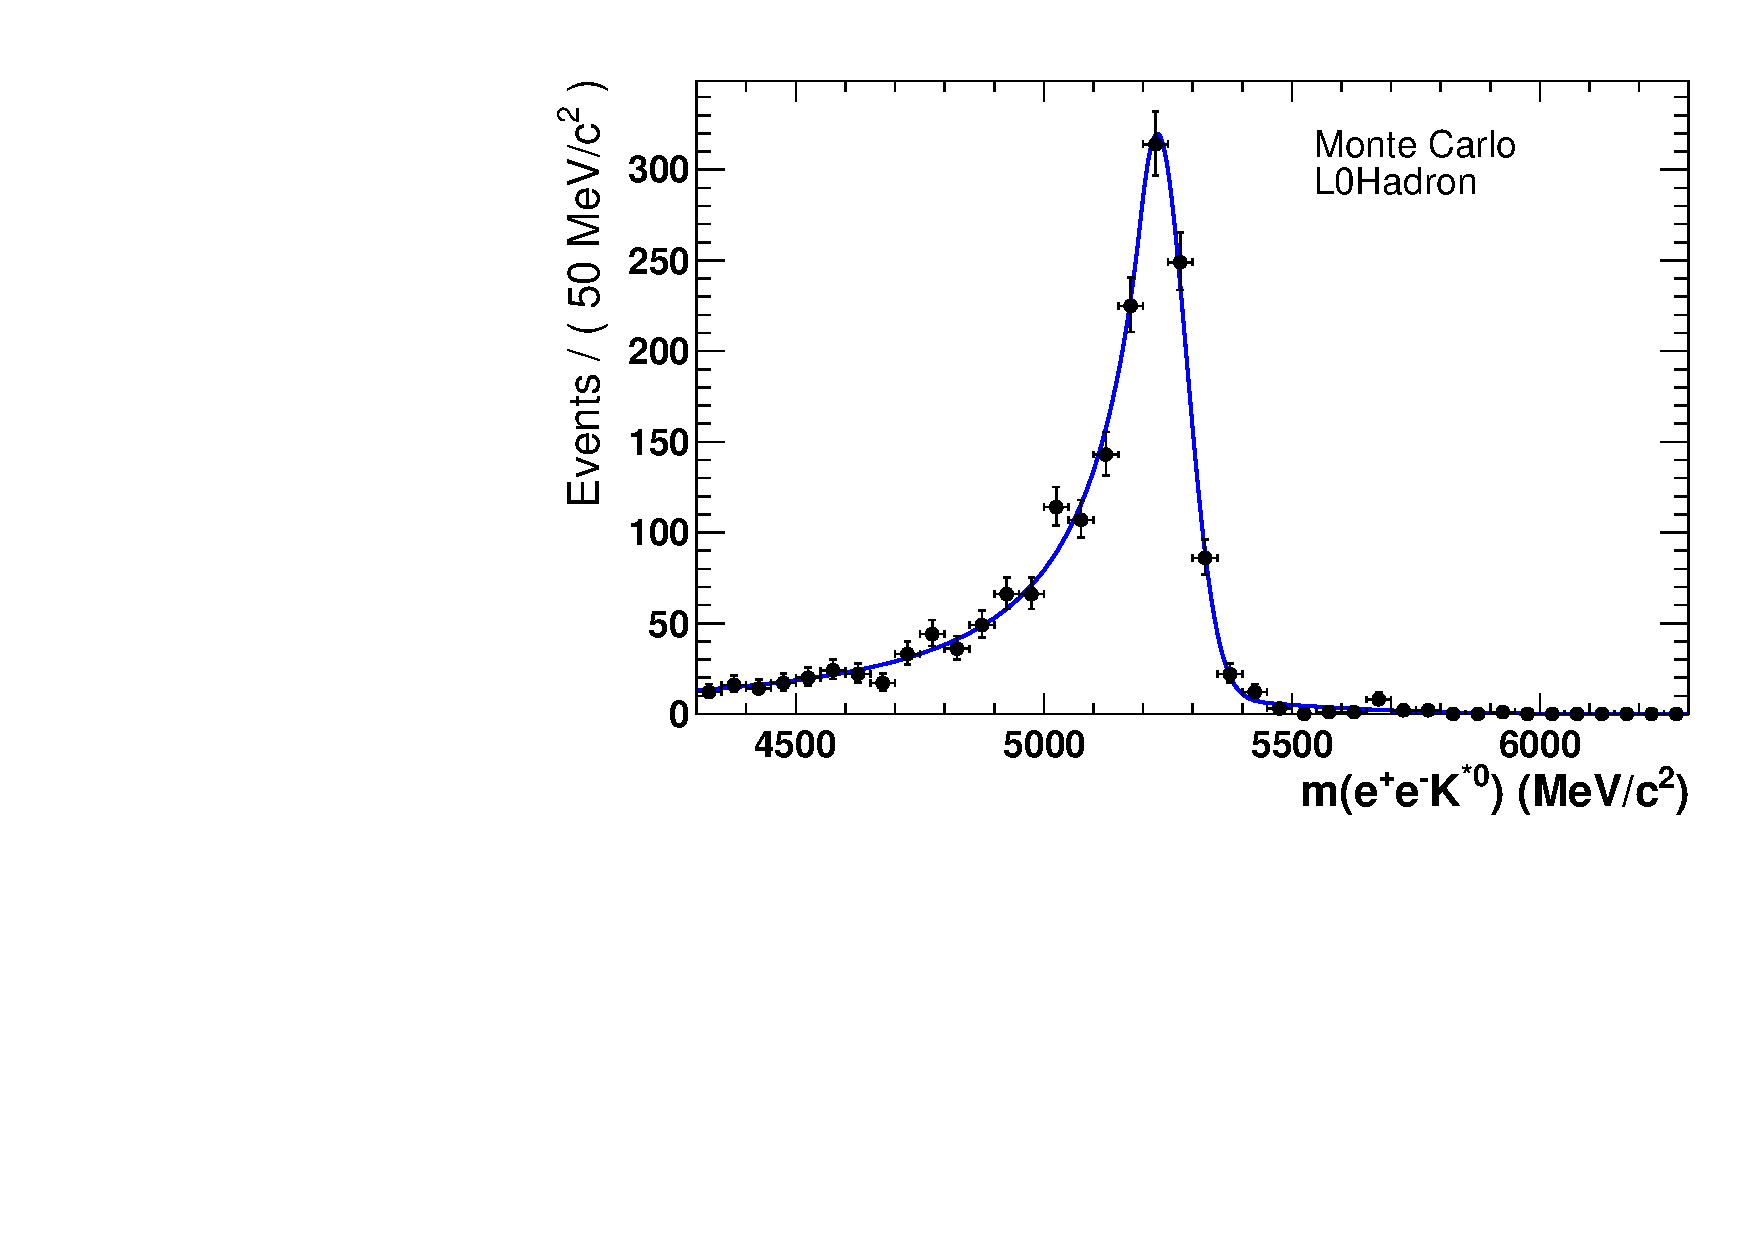
\includegraphics[width = 0.49\textwidth]{MC_L0Had_eeKstar.pdf}}
%\subfigure{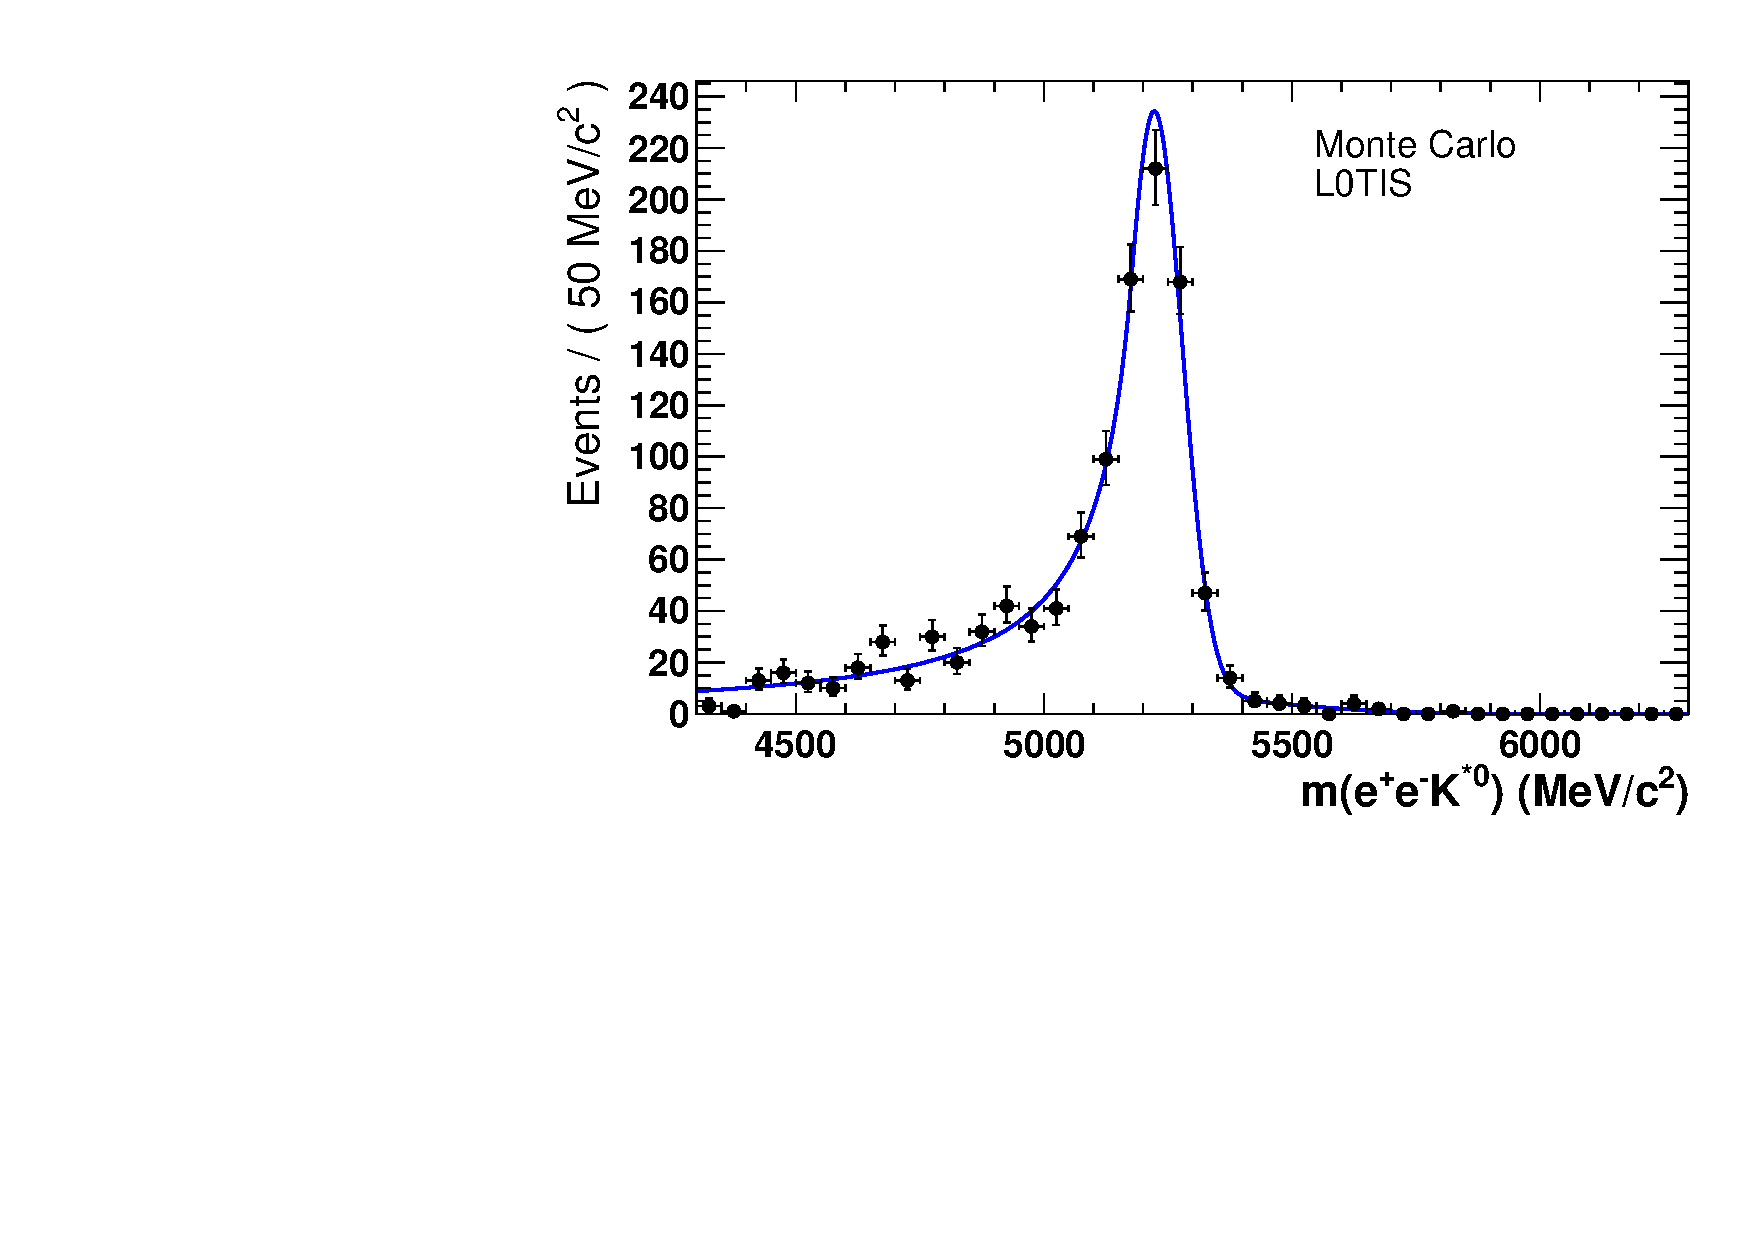
\includegraphics[width = 0.49\textwidth]{MC_L0TIS_eeKstar.pdf}}
%\end{center}
%\caption{\textit{\BdKstee Monte Carlo after the entire selection procedure. The blue curve is the fitted double Crystal-Ball distribution.}}
%\label{fig:eemc}
%\end{figure}
%
%
%\subsection{\BdToJPsieeKst \lhcb data}
%Figure \ref{fig:jpsidata} shows the \BdToJPsieeKst \lhcb data. The \PDF fitted to the data consists of the signal, the combinatorial background, the partially reconstructed background of the form $\B \rightarrow \epem Y(\rightarrow \Kstarz X)$ and the partially reconstructed background of the form $B \rightarrow (Y \rightarrow \jpsi X) \Kstarz$.\\
%
%
%
%\subsection{\BdKstee \lhcb data}
%The \BdKstee \lhcb data can be seen in Figure \ref{fig:eedata}.

%
\subsection{Results of the fit to \BdKstee \lhcb data}
Table \ref{tab:fitresults} lists the fitted parameters for the entire \PDF to the \BdKstee \lhcb data. All parameters are listed for the three mutually exclusive trigger categories. Furthermore the means by which each parameter is determined is summarised in this Table.\\
The result of the fit yields 130 $\pm$ 17 \BdKstee events selected in 3\invfb of data collected by \lhcb in the 2011 and 2012 summed over the three trigger categories. The resulting statistical signal significance of the signal obtained in this analysis corresponds to 8.3 standard deviations. \\
The number of \BdKstee signal events in this dataset is also in agreement with the number of predicted \BdKstee events calculated in the optimisation process in Section \ref{sec:opti} (see Appendix \ref{ap:SandB} for details on the predicted values). \newpage

\renewcommand{\arraystretch}{1}
\begin{table}[!h]
\begin{center}
\begin{tabular}{c|l|c|l}
parameter & L0Category & value & determined by\\
\hline
\hline
& L0Electron & 5250.1 $\pm$ 0.9 \mevcc & fit to the\\
$\mu^{data}_{\jpsi \Kstarz}$ & L0Hadron & 5231.5 $\pm$ 4.4 \mevcc & \BdToJPsieeKst \lhcb data\\
& L0TIS & 5230.7 $\pm$ 3.0 \mevcc & \\
\hline
 & L0Electron & 8.2 $\pm$ 2.7 \mevcc & difference between the means\\
$\delta_{\mu}$ & L0Hadron & -8.0 $\pm$ 8.0 \mevcc & of to \BdKstee and \\
& L0TIS &  -22.0 $\pm$ 7.6 \mevcc & \BdToJPsieeKst Monte Carlo \\
\hline
 & L0Electron & 37.0 $\pm$ 1.4 \mevcc & fit to the \\
$\sigma_1$ & L0Hadron & 58.8 $\pm$ 4.2 \mevcc & \BdKstee Monte Carlo\\
& L0TIS & 56.1 $\pm$ 3.9 \mevcc & \\
\hline
 & L0Electron & 266.7 $\pm$ 26.0 \mevcc & fit to the \\
$\sigma_2$ & L0Hadron & 280.1 $\pm$ 37.9 \mevcc & \BdKstee Monte Carlo\\
& L0TIS & 237.7 $\pm$ 34.4 \mevcc & \\
\hline
 & L0Electron & 0.87 $\pm$ 0.01 & scale factor between the widths  \\
$s_{\sigma}$ & L0Hadron & 1.05 $\pm$ 0.05 & of the \BdToJPsieeKst\\
& L0TIS &  1.02 $\pm$ 0.04 &  Monte Carlo and \lhcb data\\
\hline
  & L0Electron & 0.55 $\pm$ 0.04 & fit to the \\
$\alpha$ & L0Hadron & 0.56 $\pm$ 0.08 & \BdKstee Monte Carlo\\
& L0TIS & 0.81 $\pm$ 0.25 & \\
\hline
& L0Electron & 1.61 $\pm$ 0.11 & fit to the \\
$n$ & L0Hadron & 1.86 $\pm$ 0.35 & \BdKstee Monte Carlo\\
& L0TIS & 1.69 $\pm$ 0.43 & \\
\hline
& L0Electron & 0.96 $\pm$ 0.01 & fit to the \\
$f$ & L0Hadron & 0.92 $\pm$ 0.02 & \BdKstee Monte Carlo\\
& L0TIS & 0.91 $\pm$ 0.02 & \\
\hline
& L0Electron & 0.48 $\pm$ 0.01 & fit to the \\
$r^{part. bkg}$ & L0Hadron &  0.27 $\pm$ 0.06 & \BdToJPsieeKst \lhcb data \\
& L0TIS & 0.51 $\pm$ 0.06 & \\
\hline
& L0Electron & -0.0037 $\pm$ 0.0003 & fit to the \\
$b$ & L0Hadron &  -0.0040 $\pm$ 0.0006 & \BdKstee \lhcb data\\
& L0TIS & -0.0057 $\pm$ 0.0015 &  \\
\hline
& L0Electron & 373.5 $\pm$ 24.0 &  fit to the \\
$N^{comb. bkg}$ & L0Hadron & 104.1 $\pm$ 13.3 &  \BdKstee \lhcb data\\
& L0TIS & 85.9 $\pm$ 14.0 & \\
\hline
\hline
& \textbf{L0Electron} & \textbf{60.1 $\pm$ 11.6} &  \textbf{fit to the} \\
$\mathbf{N^{sig}}$ & \textbf{L0Hadron} & \textbf{35.0 $\pm$ 8.6} &  \textbf{\BdKstee \lhcb data}\\
& \textbf{L0TIS} & \textbf{34.5 $\pm$ 8.4} & \\
\end{tabular}
\end{center}
\caption{\textit{Parameters of the \PDF fitted to the selected \BdKstee candidates in the 2011 and 2012 \lhcb dataset after the newly developed and optimised selection.}}
\label{tab:fitresults}
\end{table}
\newpage

\section{Comparison to the results of the 2011 selection}
To quantify the quality of the selection developed in the course of this master's thesis the \BdKstee signal yield is compared to the signal yield that would have been obtained by the 2011 selection. Therefore the entire 2011 selection (including the \textit{Stripping17b} line) is applied to the \lhcb data collected in 2011 and 2012. The selected events are divided into the same three independent trigger categories as in Section \ref{sec:triggercat} and the fit procedure from Section \ref{sec:fitstrat} is applied. The results can be seen in Figure \ref{fig:oldeedata} and Table \ref{tab:comp}. The 2011 selection results in 93 $\pm$ 15 \BdKstee events selected in 3\invfb of data collected by \lhcb in the 2011 and 2012 which is about $70 \%$ of the events selected by the selection developed in this master's thesis.\\ 
The amount of combinatorial background events at very low \Bd masses in the new selection is increased with respect to the old selection. This background is removed in the old selection as a by-product of the $\Bd \rightarrow \Dm \ep \neu$ veto cut that has to be removed because of its biasing effect on the angular acceptance (see Section \ref{sec:denu}).\\

\begin{figure}[ht]
\begin{center}
\subfigure{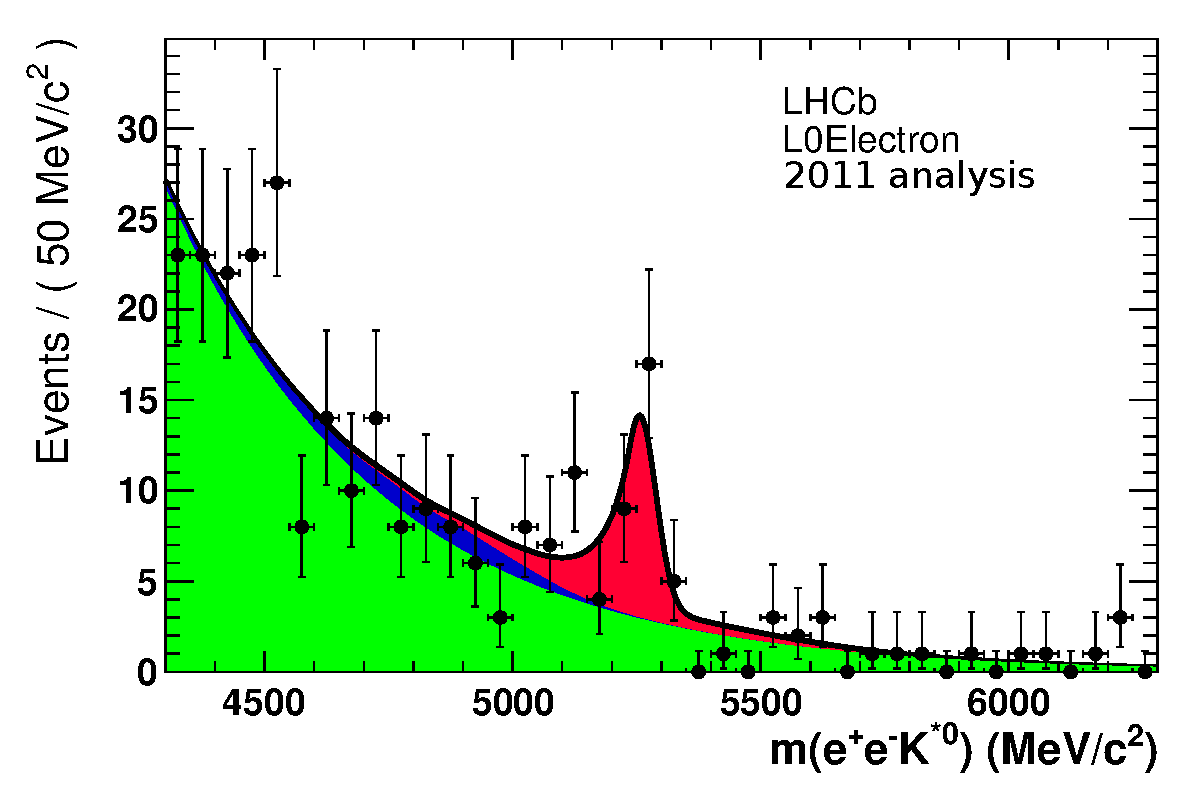
\includegraphics[width = 0.49\textwidth]{oldData_L0Ele_eeKstar.pdf}}
\subfigure{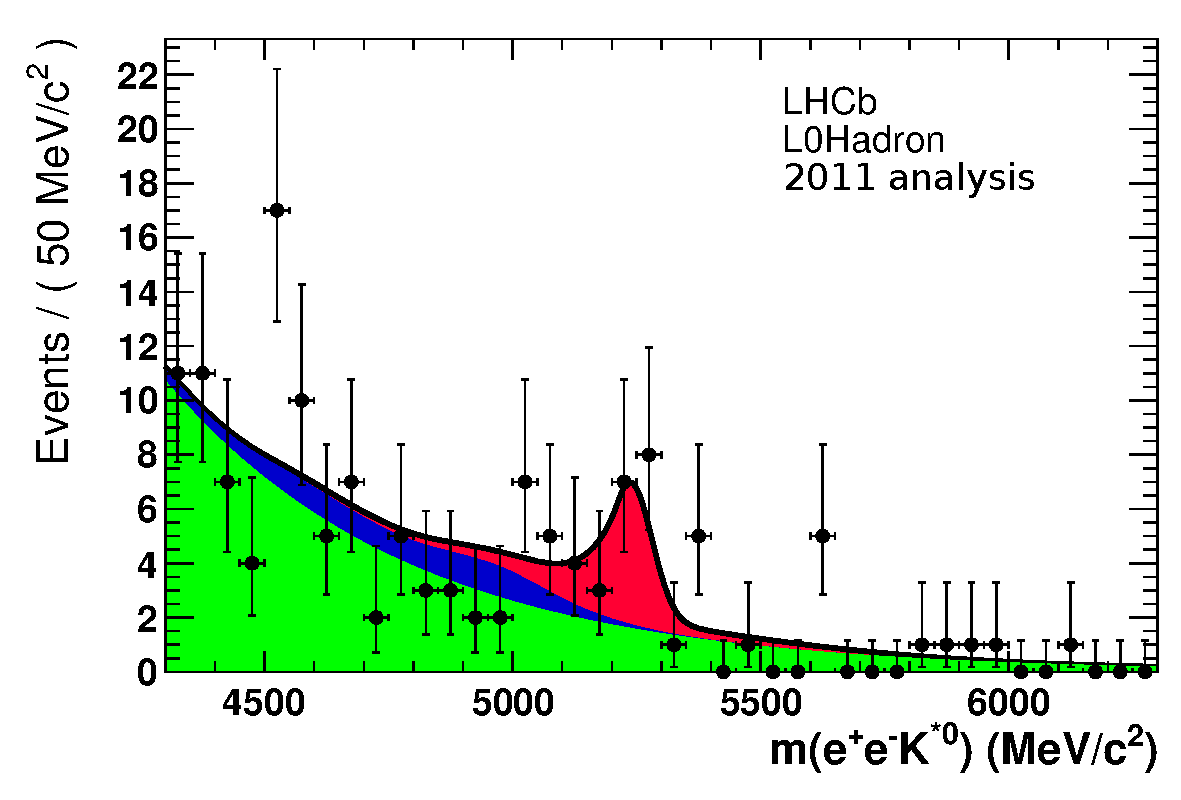
\includegraphics[width = 0.49\textwidth]{oldData_L0Had_eeKstar.pdf}}
\subfigure{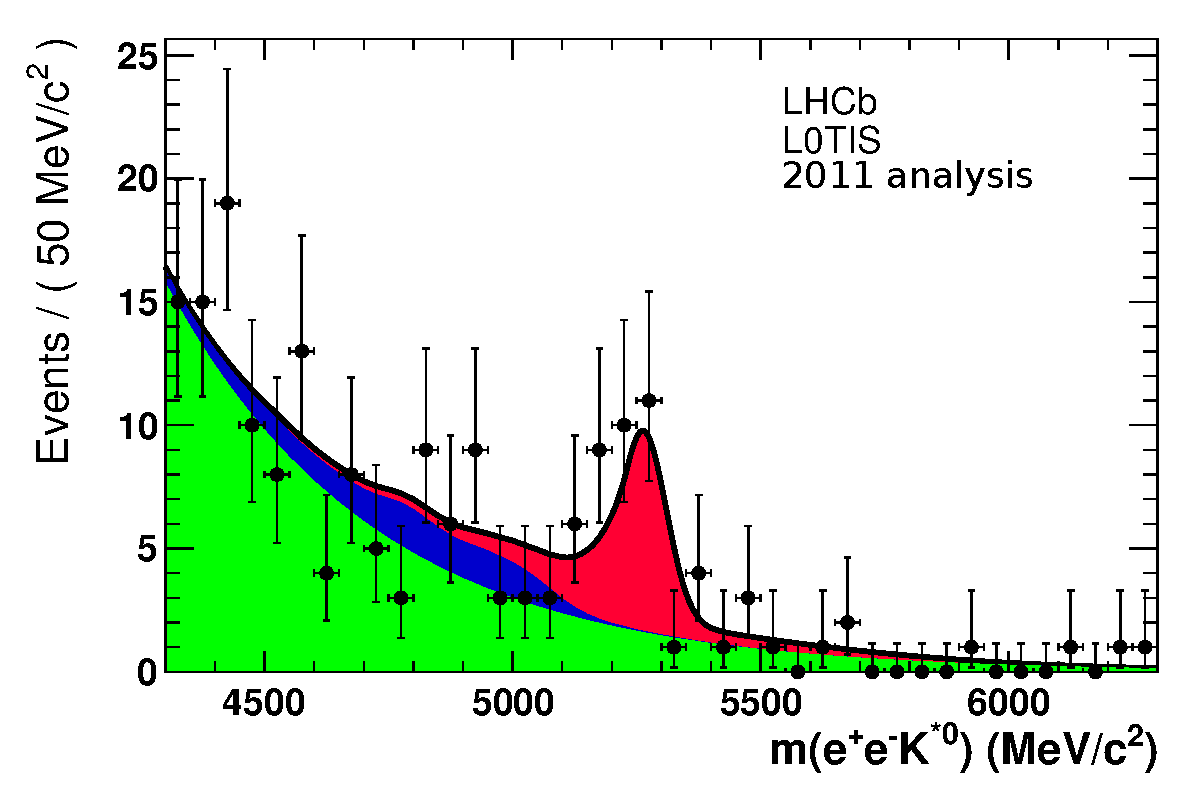
\includegraphics[width = 0.49\textwidth]{oldData_L0TIS_eeKstar.pdf}}
\end{center}
\caption{\textit{\BdKstee \lhcb data after the selection procedure developed in the 2011 analysis. \textbf{Green area}: combinatorial background events, \textbf{blue area}: partially reconstructed background events, \textbf{pink area}: \BdKstee signal events.}}
\label{fig:oldeedata}
\end{figure}

\begin{table}[ht]
\begin{center}
\begin{tabular}{c|l|c}
parameter & L0Category & value \\
\hline
\hline
& L0Electron & 35.9 $\pm$ 9.1 \\
$N^{sig}$ & L0Hadron & 21.5 $\pm$ 7.0\\
 & L0TIS &   35.1 $\pm$  9.1\\
\end{tabular}
\end{center}
\caption{\textit{Number of \BdKstee events in the 2011 and 2012 \lhcb dataset after the selection used in the 2011 analysis.}}
\label{tab:comp}
\vspace*{19cm}
\end{table}







%This \PDF is used to fit the \BdKstee and \BdToJPsieeKst Monte Carlo respectively.
%
%\subsubsection{Fit to the \BdToJpsieeKst Monte Carlo}
%The \BdToJpsieeKst Monte Carlo and the fitted signal \PDF from Equation \ref{eq:dcb} can be seen in Figure \ref{fig:jpsimc} for the three independent trigger categories. After the fit all parameters are extracted and stored.

%
%\subsubsection{Fit to the \BdToJPsieeKst \lhcb data}
%
%
%%This \PDF is used for the modelling of any signal involved in this analysis, that is for \lhcb data and Monte Carlo and for the \BdKstee decay as well as the \BdToJPsieeKst decay.\\
%%\\
%After taking into account the between the Monte Carlo and \lhcb data (for example due to imperfect detector alignment and/or effects from detector ageing that are not modelled in the Monte Carlo) the \PDF for the \BdKstee signal is expressed as:
%\begin{equation}
%\PDF^{sig} \ = \ f\ CB(x;\alpha,n,\mu + \delta_{\mu},s_{\sigma} \cdot \sigma_1) + (1-f)\ CB(x;\alpha,n,\mu + \delta_{\mu},s_{\sigma} \cdot \sigma_2)
%\end{equation}
%
%To obtain a most accurate measurement on the number of \BdKstee events all parameters of the signal \PDF are determined and fixed before the final fit.
%Therefore the double CB function in Equation \ref{eq:dcb} is fitted to the \BdKstee Monte Carlo and all parameters are extracted.
%To account for differences in resolution between the Monte Carlo and \lhcb data (for example due to imperfect detector alignment and/or effects from detector ageing that are not modelled in the Monte Carlo) a scale factor $s_{\sigma}$ is multiplied to both widths from Monte Carlo $\sigma_1$ and $\sigma_2$. Furthermore the mean $\mu$ of the double CB distributions -- which corresponds to the mass of the \Bd meson -- is given a addend $\delta_{\mu}$.\\
%% The parameter $s_{\sigma}$ is determined by using the fit result of the \BdToJPsieeKst Monte Carlo fit in the \BdToJPsieeKst data fit and letting the widths scale by $s_{\sigma}$. The parameter $\delta_{\mu}$ is the difference between the mean fitted by \BdToJPsieeKst Monte Carlo and the \BdKstee Monte Carlo. 
%The signal \PDF fitted to the \BdKstee \data is then:
%
%when $\mu$, $\alpha$, $n$, $\sigma_1$ and $\sigma_2$ are the parameters of the \PDF from \BdKstee Monte Carlo.
%\begin{table}
%\begin{center}
%\begin{tabular}{l|c}
%parameter & determined by\\
%\hline
%\hline
%$\alpha$, $n$, $\mu$, $\sigma_1$, $\sigma_2$, $f$ & \BdKstee Monte Carlo\\
%\hline
%$\delta_{\mu}$, $s_{\sigma}$ & comparison of results from \\
%& \BdToJPsieeKst Monte Carlo and data\\
%\end{tabular}
%\end{center}
%\caption{\textit{Parameters of the \BdKstee signal \PDF and the means of constraining them.}}
%\label{tab:mcfit}
%\end{table}
